\documentclass[11pt, oneside]{article}   	% use "amsart" instead of "article" for AMSLaTeX format
\usepackage{geometry}                		% See geometry.pdf to learn the layout options. There are lots.
\usepackage[parfill]{parskip}    			% Activate to begin paragraphs with an empty line rather than an indent
\usepackage{graphicx}						% Use pdf, png, jpg, or eps§ with pdflatex; use eps in DVI mode
											% TeX will automatically convert eps --> pdf in pdflatex
\usepackage{amssymb}
%\usepackage{svg}
%\svgpath{{../imgs/}}
\usepackage{comment}						% for \begin{comment}
\usepackage{pifont}							% for \ding
\usepackage{url}							% for "plainurl" support in \bibliographystyle 
\usepackage{hyperref} 						% for \hyperfootnote

% Make clickable footnote
\newcommand{\hyperfootnote}[1][]{\def\ArgI{{#1}}\hyperfootnoteRelay}
	% relay to new command to make extra optional command possible
\newcommand\hyperfootnoteRelay[2][]{\href{#1#2}{\ArgI}\footnote{\href{#1#2}{#2}}}
	% the first optional argument is now in \ArgI, the second is in #1
% Takes at most 3 parameters (see http://www.tex.ac.uk/FAQ-twooptarg.html for info on multiple optional parameters)
% If first parameter isn't given, it's value is '' (empty string in text before footnote reference)
% If second parameter isn't given, it's value is '' (string before visible URL, e.g. 'http://')
% Makes a clickable footnote (alternatively: \url{}) with optional reference in the text as well
% Use 1: \hyperfootnote{www.mywebsite.com}: creates a footnote consisting of a clickable URL
% Use 2: \hyperfootnote[My website]{www.mywebsite.com}: creates a clickable piece of text in the text ('My website') plus a footnote consisting of a clickable URL
% Note: requires the hyperref package.
% Note: use xspace package to add/absorb spaces when necessary (e.g. to avoid a space between the footnote number and a punctuation mark)
% Info on how to define a LaTeX command: https://www.sharelatex.com/learn/Commands

\geometry{letterpaper}                   	% ... or a4paper or a5paper or ... 
\usepackage{draftwatermark}
\SetWatermarkLightness{0.9}
\SetWatermarkText{DRAFT}					% you can use \today
\SetWatermarkScale{4}

\title{Identity Agents}
\author{Paul Trevithick, The Mee Foundation}
\date{March 3, 2023. Revised \today}							
\begin{document}
\maketitle
\begin{abstract}
There is a power imbalance between digital service providers and their users, with regard to these users' personal information and online identity. The result is that users lack autonomy agency. They are subjected to third-party surveillance, and are inconvenienced by today's prevailing provider-controlled, siloed architecture for personal information. We explore design considerations for potential solutions and propose a design for an on-device \emph{identity agent} and an associated legal contract, that together represent the user and protect their interests online.
\end{abstract}

\section{Power Imbalance}
While the internet has brought new services and experience to billions of people, it has also resulted in a power asymmetry between the digital service providers and their users regarding these users' digital identities and personal data. 

The internet's designers, in the interest of resilience and scalability began with a decentralized architecture that moved computation and storage to the edge of the network and minimized centralized control. However, in recent decades economic factors, so-called natural monopolies, preferential attachment network effects, economies of scale, and the relative ease of creating centralized solutions have contributed to a concentration of power in the hands of a few relatively large providers. 

Berners-Lee conceived the web as a decentralized platform wherein anyone could publish a website and link to any other site. He even envisioned that these pages would be editable. However, as the web has grown from a research-sharing community into a global medium for commerce, communication, journalism and entertainment, power has concentrated. Today, the web is dominated by enormous companies like Amazon, Meta, Google, and Netflix. These corporate giants enjoy enormous control not only over what people see and do online, but over their users' private data.\cite{Finley2017}

In response, many initiatives have arisen proposing alternative approaches and technologies. Here are just a few representative examples: \hyperfootnote[rececentralize.org][https://]{redecentralize.org}, \hyperfootnote[DWeb principles][https://]{getdweb.net/principles/}, \hyperfootnote[The Web3 Foundation][https://]{web3.foundation/}, \hyperfootnote[the Decentralized Identity Foundation(DIF)][https://]{identity.foundation}, \hyperfootnote[``local-first" software principles][https://]{inkandswitch.com/local-first/}, \hyperfootnote[ProjectVRM][https://]{blogs.harvard.edu/vrm}, \hyperfootnote[Blue Sky][https://]{blueskyweb.xyz/}, and Berners-Lee's \hyperfootnote[Decentralized Information Group][https://]{dig.csail.mit.edu}. 

We use the term \hyperfootnote[\emph{user agent}][https://]{developer.mozilla.org/en-US/docs/Glossary/User\_agent} to refer to software tools that work (i.e. provide agency) ``on the user's side"\footnote{Project VRM refers to this as ``tools for individuals to manage relationships with organizations'' to which we would add ``...or with other individuals."} for, and \emph{exclusively} on behalf of, the user. Since our discussion applies equally to a provider's mobile app, webapp, or website, from here forward we will simply use the term \emph{app} to refer to all of them.

Power asymmetry lies at the root of a diverse set of related end-user symptoms, most of which erode privacy, since privacy and power are highly interrelated concepts\footnote{Consider the title of V\'eliz's recent book, ``Privacy is Power"\cite{veliz2020}}. 
These privacy-eroding symptoms include a lack of personal autonomy, a lack of personal agency, and third-party surveillance. 

\subsection{Lack of Autonomy}

\begin{quote}
	\textbf{autonomy}: \emph{freedom from external control or influence; independence.}\hyperfootnote[][https://]{languages.oup.com/google-dictionary-en/}
\end{quote}

\emph{Independence}. In real life each of us is an independent entity. Each of us has a self that embodies our individuality. We ``bring" that independent selfness to interactions with others, with vendors, etc. while understanding that this independence is not absolute--we are still to some extent dependent on common, shared systems, laws, environments, and so on. By contrast, it has been said that ``we have no \emph{digital embodiment}."\footnote{Phil Windley, personal communication, Sepember 2022}  Our identities are provided to us by digital service providers (e.g. in the form of a Facebook identity, or an Amazon account). Without them we don't exist. Anyone who has been banned from a platform, or uses a platform that has been shut down is sharply reminded that their digital identity exists at the pleasure of that platform. Our provisional existence is the original power asymmetry. Efforts create personal datastores, or more specifically, those that strive to provide each of us a \emph{self-sovereign identity}\cite{Preukschat2021} are squarely aimed at addressing this issue--the word ``sovereignty" certainly evokes power. Lanier refers to this as a person's right to a ``First-class identity."\cite[p251]{Lanier2014}.

\emph{Ownership}. Our personal data is collected and held by organizations as we interact with their apps, but not by us. This pattern \emph{app-held data} by \emph{first-parties} is so common that it's hard to imagine an alternative. Our data is not free from external control by apps, because it is generally stored and managed by them. Our data is also collected and held by \emph(third-parties) (e.g. data brokers) with whom we have no direct interactions. In short, it's been said that \hyperfootnote[“everybody has our data … except us.”][https://]{reb00ted.org/personaldata/20210620-who-has-my-personal-data/}. 

As we'll discuss more later on, alternatives have been proposed. One is ``user-held" data\cite{Jurcys2021}, where your data is held by you in a personal datastore\footnote{Examples of open-source personal datastores include \url{https://solidproject.org}, Decentralized Web Nodes(DWN). For more about personal datastores see \url{https://wikipedia.org/wiki/Personal\_data\_service}}. Another is following ``local-first" software principles.\cite{Kleppmann2019}

\emph{Lock-in}. As we've mentioned our online existence is provisional. Our existence is bound to the provider from which it originated. Providers hold our data, and although in many jurisdictions providers are required to allow us to have access (e.g. to request that we can download a copy), we lack the technical means to accept the data stream and store it under our control (e.g. in a personal datastore). If we did we'd have the potential to subsequently transform it into other formats and thereby make it reusable in other contexts. Thus our data is held hostage, i.e. without autonomy. 

\emph{Peer-to-peer}. With a few exceptions\hyperfootnote[][https://]{berty.tech}, internet users, when they communicate person-to-person don't have the ability to do so \emph{peer-to-peer}--from their edge device to the other person's device. Instead, they are dependent on servers hosted by intermediaries. Whereas it is now standard practice that the content of messages is end-to-end encrypted, the metadata about them (e.g. who a person communicates with, from where, at what time, how often and from which device, etc.) is in many cases visible to the intermediary server. 

\subsection{Lack of agency}

\begin{quote}
\textbf{agency}: \emph{the capacity, condition, or state of acting or of exerting power} \hyperfootnote[][https://]{www.merriam-webster.com/dictionary/agency}
\end{quote}

\emph{Wielding credentials}. In real life you can present your drivers license to a wine seller in order to prove that you are of drinking age since the wine seller trusts the license issuer. The interaction is privacy-respecting because the presentation interaction is not disclosed to the issuer. This could be described as \emph{wielding} a trust credential. At present, there is no equivalent way to do this online. There's no standard way to be issued a credential, hold it in digital wallet, and then present it. With a few, domain-specific exceptions (e.g. cryptocurrency), there is no standard online method for you to prove something one party states about you, to another party.

\emph{Data presentation}. One reason providers' apps rely on form filling and other kinds of data entry is that the user, even one equipped with a personal datastore, lacks the ability to present personal information digitally to the provider. Instead, the information must be re-entered manually at each provider. The credential presentation interaction mentioned is another example of this.

\emph{Delegation}. In the offline world one entity can grant access to some resource to another entity. For example, I can give my car keys to a friend so they can borrow my car. There is no standard, secure way to do this online. This is especially problematic in healthcare scenarios where a healthcare provider needs access to electronic health-related data about a patient, whereas the patient may not be able to provide it by themselves but instead needs to rely on someone else, e.g. a family member to grant the needed permission.

\emph{Privacy self-management}. Today, despite significant new regulation, the basic approach to protecting privacy hasn't changed since the 1970s. It is often called \emph{notice \& consent}. Solove described it using the term \emph{privacy-self management}\cite{Solove2012}, as follows:

\begin{quote}
	[T]he law provides people with a set of rights to enable them to make decisions about how to manage their data.  These rights consist primarily of rights to notice, access, and consent regarding the collection, use, and disclosure of personal data. The goal of this bundle of rights is to provide people with control over their  personal data, and through this  control people can decide for themselves how to weigh the costs and benefits of the collection, use, or disclosure of their information.
\end{quote} 

Although well-intended, and necessary, \emph{notice \& consent} does not provide people with meaningful control over their data. The problem is well summarized by \cite{Flanagan2020}: 

\begin{quote}
	When presented with click-through consent, privacy policies or terms of use statements, most people reflexively select “I agree”. An extensive body of academic research specifically on privacy and data collection notices demonstrates that members of the public don't read them and might not understand them if they did and that many misinterpret their purpose, assuming that the existence of a privacy policy displayed by way of notice means that the entity collecting the data offers a level of data protection when, in fact, privacy notices do not guarantee privacy. Since the terms offered are typically “take it or leave it”, to decline often results in being denied the product or service one seeks, creating a disincentive for consumers to do anything other than accept the terms.
\end{quote}

Even if it were cognitively feasible for an interaction with a single entity's app(s), the sheer number of entities collecting and using personal data makes it infeasible for people to manage their privacy separately with each. Privacy-self management doesn't scale from the individual's point of view. They lack agency (i.e. human-centic computational capability) necessary to perform the required tasks.

\emph{Privacy policy expression}. With a few exceptions, (e.g. the \hyperfootnote[Global Privacy Control][https://]{globalprivacycontrol.org}), users  lack the technical means (i.e. computational capability) to express their own privacy terms to providers. 

\emph{User rights}. In a growing number of jurisdictions, including Europe under \hyperfootnote[GDPR][https://]{gdpr-info.eu/} and California under \hyperfootnote[CPRA][https://]{thecpra.org/}, the user's data rights, (e.g. the right to access, correct and delete their data), are clearly described. In principle these laws respect these rights, however in practice the time and effort required to exercise these rights at every app is sufficiently onerous, that in practice they are not respected. The user must send written requests to get copies of their data, update it, or have it be deleted. The power of user agents is necessary to regain in practice, the rights they already have in principle. 

\emph{Content filtering}. Social networking platforms have replaced human content editors with algorithmic filters. Users might think that they see a balance of content whereas in reality they are trapped in what Pariser called ``filter bubbles."\cite{Pariser2011} Pariser's recommendation is that if platforms are going to be gatekeepers, they need to program a sense of civic responsibility into their algorithms, they need to be transparent about the rules that determine what gets through the filter, and ``they need to give user control of their bubble."\cite[p66]{McNamee2020}

\emph{Behavioral advertising}. Behavioral, (aka targeted) advertising involves the automatic generation of interest profiles by third-party adtech firms. In most cases users have no control over these interest profiles, and no ability to correct them.

\subsection{Third-party surveillance}

Whereas the user is at least aware when they sign up on a first-party app that their interactions are known to the provider of that app, there are also hundreds of third-parties of which the user is unaware that track and assemble databases about them. Databases of user data in the hands of hundreds of unknown third-parties creates privacy risks and vulnerabilities. Users have no visibility into what's being gathered, where it's being shared, and how it's being used. It is worth noting that that much of this third-party tracking is enabled in collaboration with first-parties (e.g. first-parties placing third-party tracking cookies on the user's browser).

\emph{Surveillance-based targeted advertising}. Targeted advertising \footnote{Also known as behavioral advertising, or more recently, interest-based advertising} involves four main processing steps: (i) the collection of observations about the user by a first- or third-party, (ii) synthesis of an ``ad profile” from these observations, (iii) matching this ad profile against available ``target audiences”(i.e. characteristics of whom the advertiser wishes to reach, advertising budget, etc.) from advertisers through a bidding process, and (iv) displaying the winning ad. What many people find objectionable is \emph{Surveillance-based} targeted advertising wherein step (i) above is achieved by third-parties who track the user as they move from app to app and site to site across the internet (using third-party cookies, newer, cookie-less alternative identifiers, and other tracking mechanisms). 

\emph{Data brokers}. Data brokers are third-parties who buy and sell personal data to other brokers, to advertisers, adtech firms and first-party publishers. They provide personal data marketplaces behind the users's back. They could be considered an unfortunate, privacy-invading \emph{iterim} solution to address the fact that users lack user agents with which to directly provide this data about themselves. 

\subsection{Inconvenience}
In the prevailing architecture of the internet each ditial service provider manages their own information ``silo" of information about the user (i.e. their account). This approach and the lack of sufficiently powerful user agents creates inconvenience.

\emph{Repetition}. When using apps, users are often asked to provide information about themselves that another app has already asked them, such as ``what is your email address?" This is a symptom of the internet's silo-ed architecture wherein each app maintains its own database of personal information. The user has the hassle of repeated data entry, and the app offers a less-than-optimal user experience.

\emph{Password management}. The average user uses roughly 100 websites and 25 apps daily. Although managing and periodically updating strong, unique passwords at each is impractical without an automated password manager user agent, it has been estimated that less than five percent of internet users use one. 

\emph{Account management}. The user shoulders the burden of maintaining the timeliness and consistency of their account information at hundreds of apps. For example, updating contact or credit card information at each is tedious, time-consuming and encourages the user to spend more time at sites that already have their information. The relative convenience of shopping on Amazon vs. other e-commerce sites is a consequence partially caused by the user not having a user agent to manage these relationships.

\section{Design Considerations} %Design Considerations

In this section, we discuss design considerations for a solution aimed at addressing the symptoms described in the previous section.

\subsection{Human-centricity}

Many of the challenges described thus far have their origin in an architecture that is \emph{provider-centric} rather than \emph{human-centric}. The internet is comprised of millions of providers, each offering their own app[s]. In this provider-centric model each provider's app sees a narrow slice of the individual through the lens of their direct interactions with that user. 

For the individual the situation is reversed. They sit at the center of a hub with many dozens of connections to apps radiating outwards from them. Even for a single app there is considerable burden for the user to enter and update personal information, payment details, and preferences, and review privacy policies, and set cookie preferences, and so on. Multiplied by perhaps one hundred connections the resulting burden is practically impossible. 

Tools to manage these chores must sit on the user's side and on their behalf across all of them. Technologies of this kind, that empower the user across multiple apps, e.g. browsers and password managers, are called are \emph{user-agents} since they act as agents of the user. 

\subsection{On-device storage and processing}
If we assume a human-centric decentralized architecture, where should the user's personal datastore and associated processing live? Should it be on-device or in the cloud? By on-device we mean that the primary location for a user's datastore and processing is on their own phones, laptops, and perhaps home servers. Cloud-based means that the user's datastore and processing lives primarily in the cloud (e.g. on a \hyperfootnote[SOLID][https://]{solidproject.org} pod). We say \emph{primarily} because there are usually use-cases that involved replicating/syncing some of the data to the ``other" location. 

\emph{Security}. Although this is debatable, it is our contention that given a large number of users, having a personal datastore on-device is more secure than in the cloud. Even if each alternative were equivalently secure for a single user, a cloud-based architecture by its very nature aggregates large numbers of personal datastores at one cloud service provider location and thereby creates a much larger economic incentive for hackers. 

\emph{Equity}. Any solution must be able to be afforded by all socio-economic classes and not just those better off. For this reason, we believe solutions that incur monthly hosting fees are disqualified. Since users own their devices and can ``host'' new apps there, the situation is better, although there is a cost for the additional storage required for an on-device datastore.

\subsection{Replication}

If we assume an on-device personal datastore, we introduce the need to solve the related, so-called \emph{roaming} problem. That is, we must support use cases wherein the user has more than one device that are intermittently connected to the internet and needs to have their datastore state be consistent across these devices, at least eventually. This requires that the user's agents implement data replication and syncing between themselves. An open research question is how to achieve this replication without the need for relay servers and their attendant costs which undermine the equity consideration previously mentioned.

\emph{Backup}. One disadvantage of so-called \emph{non-custodial}, on-device architecture (as compared to cloud-based architectures) is the vulnerability of users who are not diligent about backing up their devices (e.g. to an online service) to losing their agent-managed personal data. For users with more than one device this is less likely since data is replicated (as mentioned above) across their devices, and a repaired or replaced device's data can be restored from one of the user's other devices. There remains of course the worst-case scenario wherein the user hasn't backed up any of their devices and all of them are lost or damaged simultaneously. 

\subsection{Loyalty}

Much of the power asymmetry described in the first section is due to economic incentives for providers to motivate them do just enough in the user's interest to keep them as a user or customer, but not more. Personal data, after all, is considered by business to be an asset class and thus the more of it that is collected and monetized the better. If an agent is to work \emph{exclusively} on behalf of the user, the agent provider must not have an economic incentive to provide anything less than complete loyalty to the user's interests. 

Although there are other potential solutions (e.g. data cooperatives and data unions) one of the simplest is that the agent provider be a nonprofit organization that has no economic interest in the user's data. This being the case, there is no need for the agent provider to have any access to the user's data.

\subsection{Metacontextual}

Zuckerberg once said that ``[h]aving two identities for yourself is an example of a lack of integrity"\cite{Kirkpatrick2011}. However, even if one could force all users of a single system (e.g. Facebook) to have a single identity, this approach is clearly unworkable for a solution that represents the user across multiple, widely varying systems and contexts. People need the freedom to be themselves--selves that are complicated and messy. Our identities vary depending on whom we are interacting. We choose to express different parts of ourselves within different contexts. Not only are the attributes we share different the values of one attribute may be different in different contexts. 

\begin{quote} ``[A]t various times in the same day, virtually every adult can be a friend, a worker, a supervisor, a citizen, a mentor, a student, a musician, a customer, a lover, a child and a parent. Each of these roles demands different behavior and different aspects of our selves, aspects that need not be consistent. We behave, for example, in different ways with loved ones than with those we encounter in commercial or professional settings. Even among our loved ones, we behave very differently (and often show very different sides of ourselves) to our children, our parents, and our sexual partners. But this is not dishonest, nor is it inconsistent. At the very least, it's no more inconsistent than is the complicated nature of having a self. It is human."\cite[p122]{Richards2021}
\end{quote}

Let's look at a person's age as an example. We see that across contexts they might share, their exact chronological age among their close friends, a fictional age to a music recommendation service, no age at all in contexts wherein doing so might cause discrimination against them, or a merely a statement that they exceed the legal drinking age. 

In his \hyperfootnote[last public speech][https://]{www.youtube.com/watch?v=9DExNTY3QAk}  
\hyperfootnote[Kim Cameron][https://]{en.wikipedia.org/wiki/Kim\_Cameron\_(computer\_scientist)} introduced two useful definitions based on archaic English:

\begin{itemize}
\item \textbf{Selfness}: The sameness of a person or thing at all times or in all circumstances. The condition of being a single individual. The fact that a person or thing is itself and not something else. Individuality, personality. 
\item \textbf{Whoness}: Who or what a person or thing is. A distinct impression of a single person or thing presented to or perceived by others. A set of characteristics or a description that distinguishes a person or thing from others. 
\end{itemize}

Figure~\ref{fig:multiple-contexts} illustrates these concepts and introduces the notion of context.

\begin{figure}[htbp]
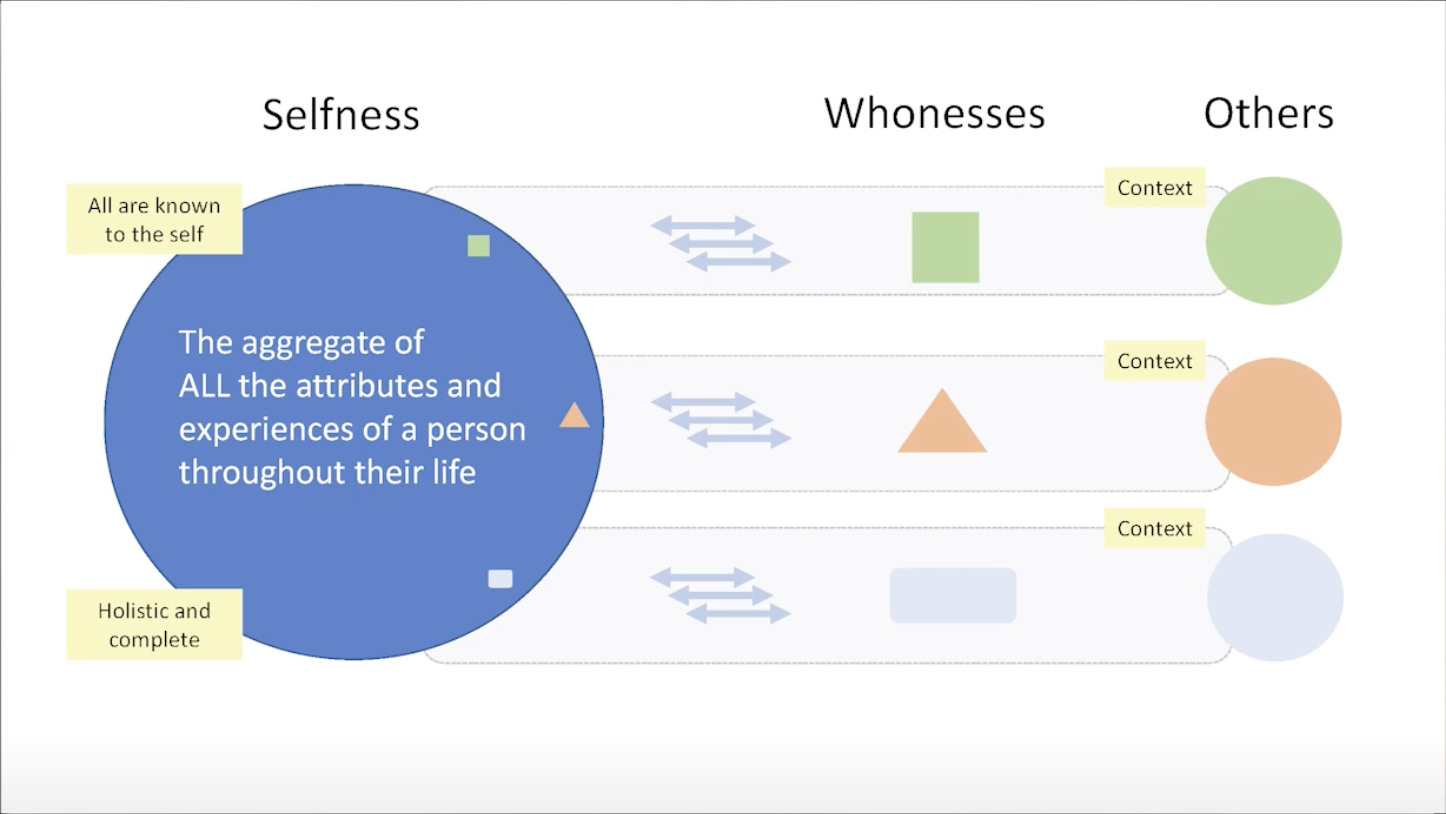
\includegraphics[width=\textwidth]{./images/selfness-and-whoness-larger.png}
\caption{Multiple whoness-contexts around a single selfness}
\label{fig:multiple-contexts}
\end{figure}

Using these terms we can say that in everyday life people have one \emph{selfness}, but they have many, context-dependent \emph{whonesses}. Any solution must be metacontextual--it must embrance and explicitly support the complicated, multi-contextual nature of our lives.

\subsection{Delegation}

In \emph{A Human Rights Approach to Personal Information Technology}\cite{Gropper2022} Gropper asserts that there is an architectural principle that must be adhered to in order to respect human rights [e.g. to privacy]. He identifies three universal components:

\begin{itemize}
\item \textbf{Authentication} (signing-in and signing documents)
\item \textbf{Request} for information (e.g. forms, searches, conversations)
\item \textbf{Storage} (e.g. labs, prescriptions, social contracts, transactions [, other human information])
\end{itemize}

The then asserts what could be called the \emph{Gropper Principle} as follows (our words, his ideas):
\begin{quote}
``Any system that respects the human right to privacy must not bundle authentication, request, and storage."
\end{quote}

In his presentation\hyperfootnote[][https://]{identiverse.com/idv2022/session/841489/} at the 2022 Identiverse conference provides additional detail (see \hyperfootnote[slides][https://]{drive.google.com/file/d/1lwaMVkG4kLi7z6cXhqMx-DGkUww9azW3/view}). It explains that only a decentralized architecture can implement the Gropper Principle because each of the three components needs to be implemented separately. For this to work in an open world with multiple alternative component providers, there will need to be a convergence on open standards between these three components. 

\subsection{Trustworthiness}

Any agent solution for online identity is by it's nature managing highly sensitive information. In order to be adopted voluntarily by people any solution must be trustworthy--its users must have confidence that their information isn't being used against their interests. 

Solutions based on open-source software can leverage transparency to help build this confidence that the solution is trustworthy. In open-source software the source code is visible to anyone to review and audit to ensure that the solution is secure, free from vulnerabilities, and works in the user's interest.

In addition to open-source, users will also consider the nature of the organization offering the solution as to trustworthiness. The organization's financial incentives should be aligned with their users' interests. In this regard a nonprofit organization can be created that has no financial or business incentive to exploit the user's data against the user's interest. Ideally the organization would have no need to have any access to the user's data so that there's simply no reason to have to trust them, their security infrastructure, and practices.

\subsection{Data Governance}

Once data is shared from the agent to a first-party there are no technical means to constrain what the recipient can do with it. No technical means, for example, can prevent them from selling it others. Instead, legal means must be employed. Existing privacy regulation is insufficient, so we propose that first-parties sign a Human Information License (HIL) to license the user's information. The HIL terms are fair and balanced, and respect the user's privacy rights. This contract is signed by a trusted organization\footnote{These kinds of organizations have been variously described in the literature as ``data unions,'' ``data coalitions,'' ``Mediators of Individual Data" (MIDs) by Lanier et al.\cite{Lanier2018}, etc.} that represents the community of identity agent users thereby making the processes effortless for them. Lasly, this organization is responsible for enforcement of the contract's terms, again, on behalf of the individual user.

\subsection{User rights}

People should enjoy user rights to access, correct and delete their own personal information managed by providers. Privacy regulation provides these rights in theory, but the user's chores to exercise these rights across hundreds of apps is unmanageable in practice. Users need user agents that can automate these processes, to reduce the amount of work to a practical level. 

\section{Identity Agents} 

In this third section we propose a solution to the problems described in the first section that is consistent with the design considerations in the second. Our solution which we call an \emph{Identity Agent} is a trusted, personal user agent\footnote{Similar ideas have been proposed by others. See \emph{personal user agents}, in \cite[p24]{Flanagan2020}} that manages a person's online identity and personal information. 

\subsection{End-user perspective}
An \emph{identity agent} is kind of user agent that gives the user control (power) over their own personal information as they interact with websites, mobile apps, and other user's agents. It does this through a combination of technical and legal mechanisms.

\subsubsection{Privacy and Autonomy} 
The agent is installed as an app and runs on the user's edge devices (mobile phone, laptop, etc.) where, entirely under the user's control, it maintains a local, private database of the user's personal information. When an app wants to know something about the user, the agent shares as much or as little as the user chooses. If an app signs a Human Information License and thereby becomes \emph{certified}, the legal entity behind that app is thereby obligated to (i) require explicit consent for collection, processing, storage and sharing of the user's data and to (ii) implement APIs to exercise the user's rights to access, correct and delete the user's personal information. We envision that agents could provide ad profiles to certified publisher websites that are supported by interest-based advertising while eliminating the need for surveillance by third-parties.

\subsubsection{Convenience}
Although the agent is an interactive application, it operates in the background most of the time. Always working solely in the user's interest, it collects information from apps that already hold their data and shares it with other apps that need it. Our vision is that that the user \emph{never has to repeat themself} (nor remember passwords!) as they move from app to app across the internet.

Here are a few examples. If an app wanted to know the user's email address, it might ask for it in a web form. In this case the agent would use its form-filler ``protocol" to fill in the value. If the app supports password-less sign-in (e.g. using OpenID Connect) the agent acts as the identity provider. If an app needed a digital driver's license credential, the agent acts as a digital wallet and presents this credential that it had presumably downloaded earlier from an issuing app. In these different examples, different protocols for information sharing would be used, and the agent must be technology agnostic and support all of them. Only in this way an agent be human-centric and put the one user at the center of all of their online relationships.

\subsection{Self and contexts}
The agent represents both the user's single \emph{selfness} and their multiple context-dependent \emph{whonesses}.

The selfness of the user is held in a data container called the \emph{self}. The contents of the self are holistic and therefore quite sensitive. For this reason, they would normally not be shared in a direct or comprehensive form with others. The user's self is the point of integration across contexts each of which may be from differing identity systems, use different protocols for communication and different schemas for knowledge representation.

Each context is represented by a \emph{context} data container. A directed \emph{correlation} link points from an entity in the self to the entities representing the user in each context. To ensure privacy only the user knows that each of these separate contexts contain representations of them. Each context represents an interaction via some communications protocol with an external app, website or agent. 

We can illustrate these concepts with a simple example. A user might play a game on a gaming app using the id DevilSpawn666, while communicating on Twitter as @alicewalker and subscribing to the New York Times as alice.walker@gmail.com. Figure~\ref{fig:three-contexts} shows a simplified view of how this is represented:

\begin{figure}[htbp]

\includegraphics[width=\textwidth]{./images/example1.png}
\caption{Alice with three contexts}
\label{fig:three-contexts}
\end{figure}

\subsection{Functionality}

Figure~\ref{fig:functionality} shows a summary of the functionality of an identity agent.

\begin{figure}[htbp]
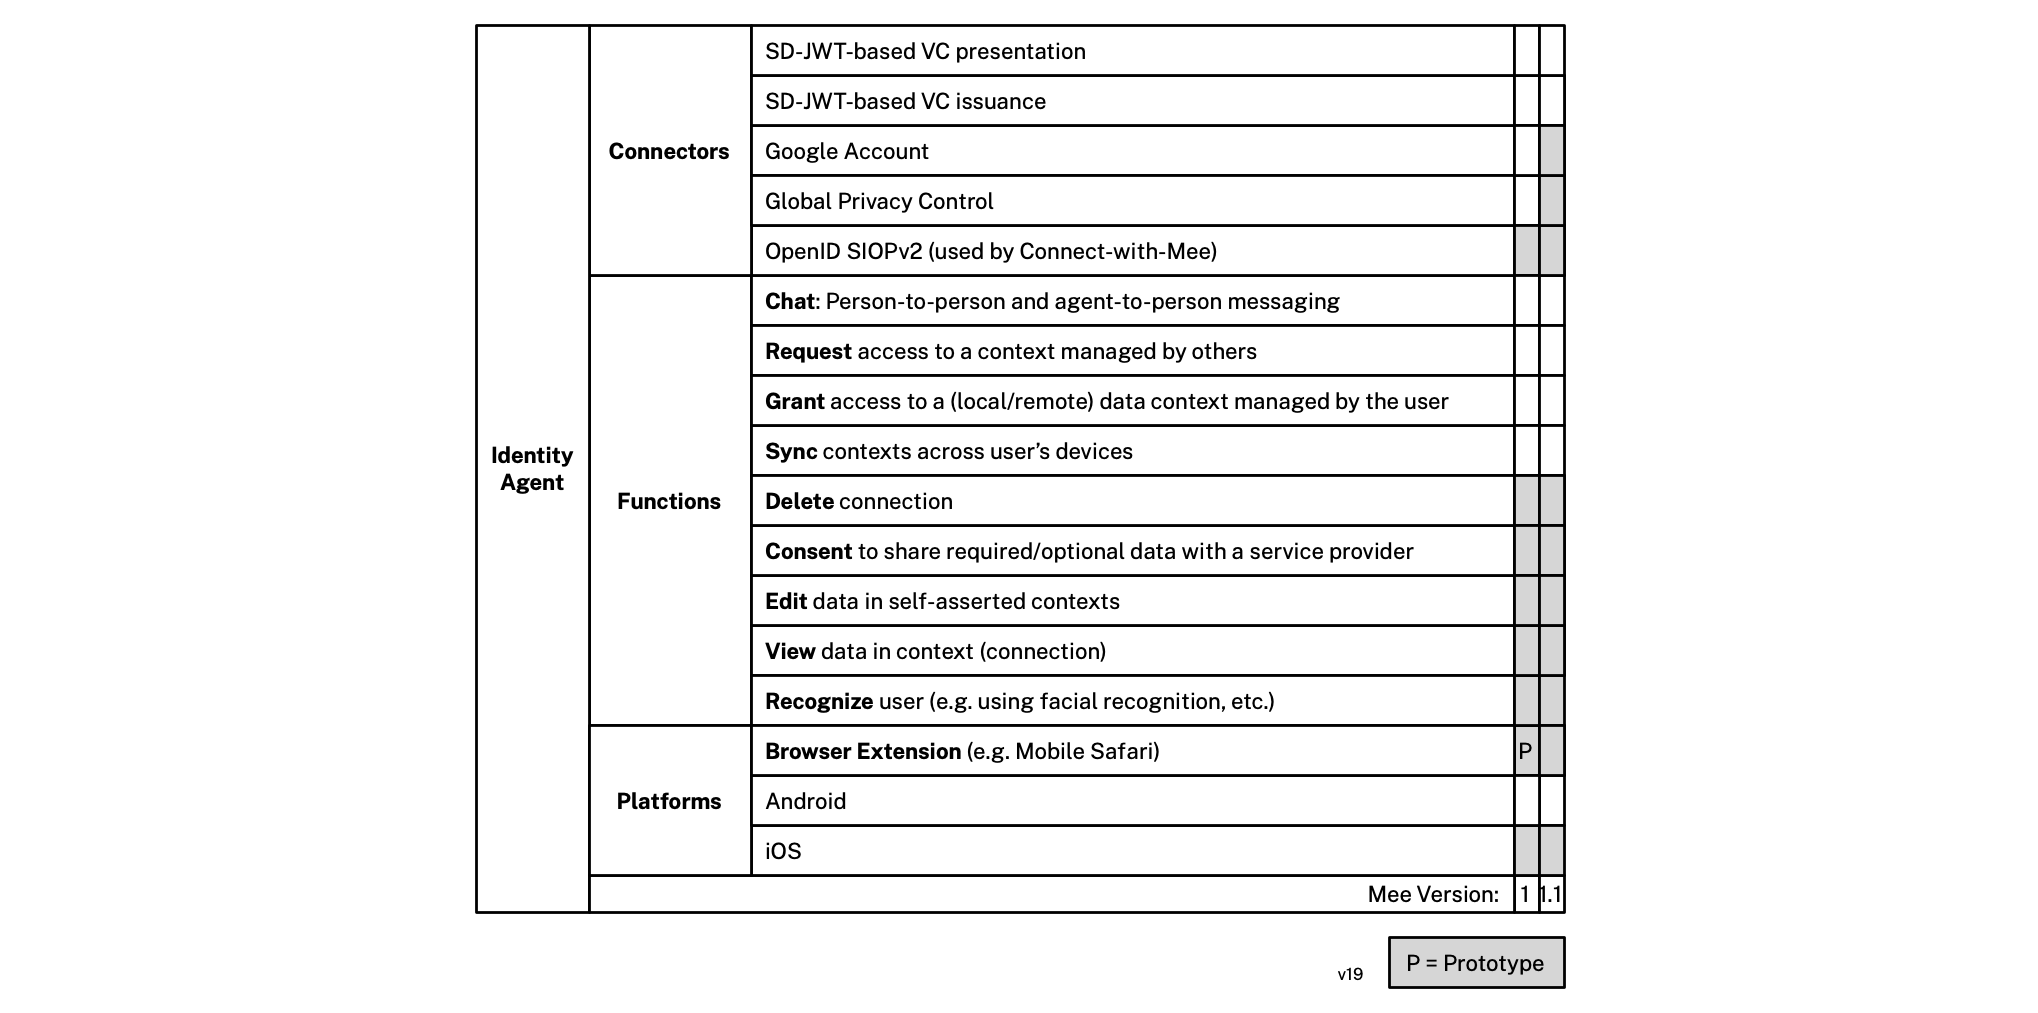
\includegraphics[width=\textwidth]{./images/agent-functionality.png}
\caption{Identity agent functionality}
\label{fig:functionality}
\end{figure}

\subsubsection{Protocols}

\begin{itemize}
\item SD JWT-based VC presentation
\item SD JWT-based VC issuance
\item PassKeys (WebAuthn)
\item Global Privacy Control
\item Connect-with-Mee: (OpenID SIOP) that uses a universal link to the agent
\end{itemize}

\subsubsection{UI Features}

\begin{itemize}
\item \textbf{VC Wallet:} import, store, manage, and present Verifiable Credentials (VCs). Note: the [OWF conceptual architecture](https://github.com/openwallet-foundation/architecture-task-force/blob/main/docs/architecture/conceptual-architecture.md) adds Burn, Receive, Send, Transfer, Refund, Purchase, Withdrawal, Deposit
\item \textbf{Recognize} user (e.g. using facial recognition, etc.)
\item \textbf{Consent} to share required/optional data with a service provider
\item \textbf{Edit} data in self-asserted contexts
\item \textbf{Chat:} Person-to-person and agent-to-person messaging
\item \textbf{View} data in contexts
\item \textbf{Delete connection} delete all data associated with this set of contexts
\item \textbf{Request} access to a context managed by others
\item \textbf{Grant} access to a (local or remote) data context managed by the user
\item  \textbf{Restore:} recover all data using SRP and backups
\item \textbf{Backup} local contexts
\item \textbf{Sync} contexts across user's devices
\end{itemize}

\subsubsection{Components}

\begin{itemize}
\item \textbf{Authorization Server}: GNAP AS
\item \textbf{Replication}: synchronization of context state across the user's set of agents
\item \textbf{Messaging}: communications among members of the user's set of agents
\item \textbf{Storage}: local data storage for contexts  
\end{itemize}

\subsection{Architecture}

In this section we propose an architecture for identity agents. We consider a user, Alice, and her agent's three layered architecture shown in figure~\ref{fig:architecture}.
\begin{figure}[htbp]
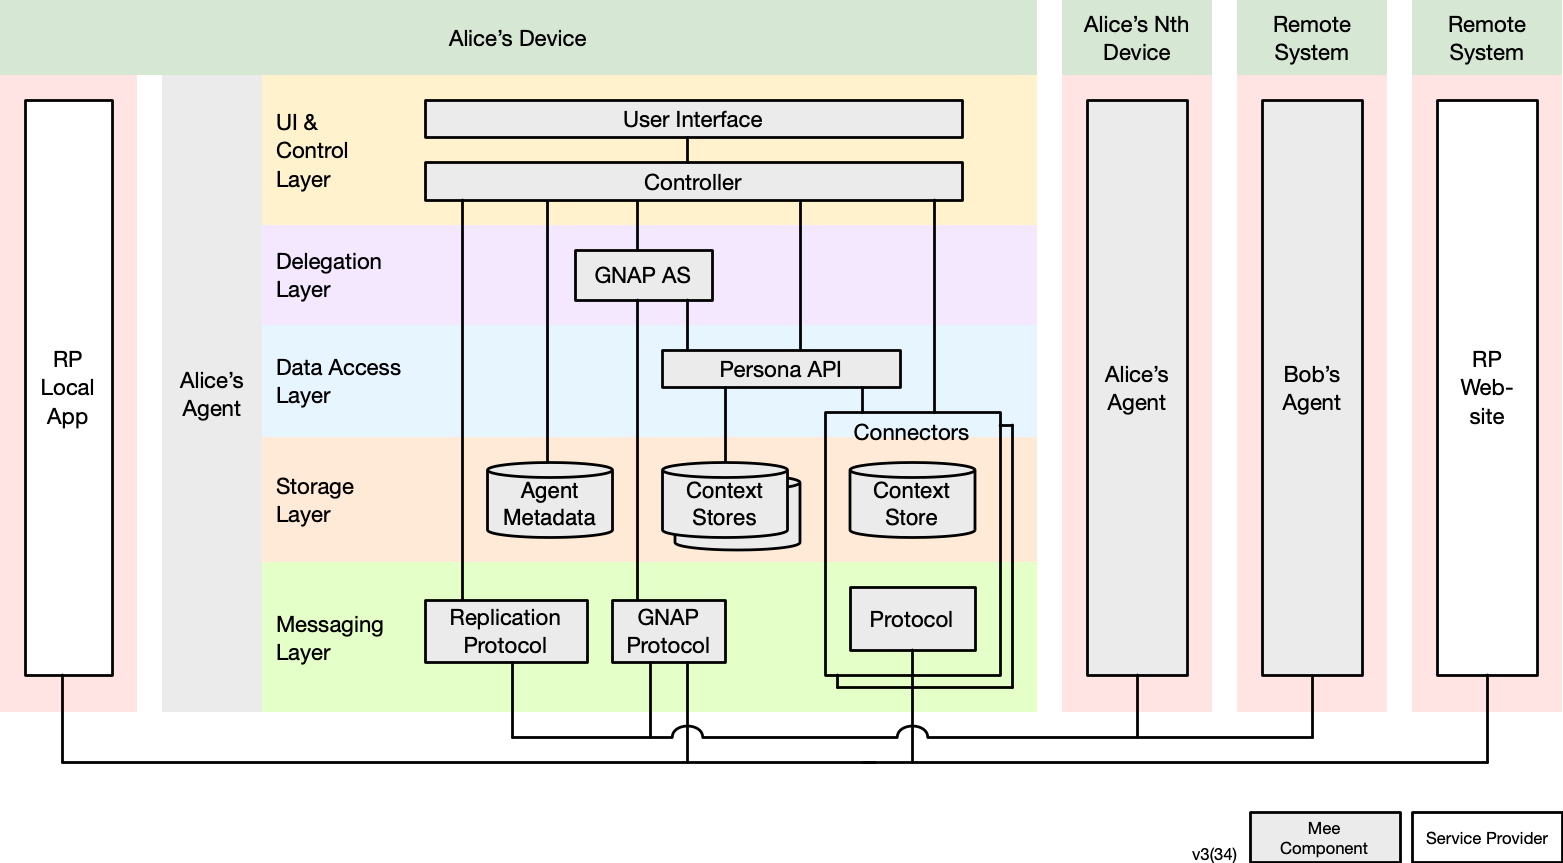
\includegraphics[width=\textwidth]{./images/architecture.png}
\caption{Architecture}
\label{fig:architecture}
\end{figure}

\subsubsection{UI layer}

Alice's identity agent is deployed as an app on Alice's device (e.g. a smart phone). The top, UI layer provides Alice with data management features to connect with apps/sites and manage her data. This UI allows her to inspect, and in some cases, edit each of the partial representations of her in each connection's context(s). Part of this UI is an "agent facade"--a presentation layer for how Alice appears to other agent users. 

\subsubsection{Delegation layer}

The \hyperfootnote[GNAP][https://]{oauth.net/gnap/} Authorization Server (AS) responds to requests for access to Alice's context datastores wherever they may be located physically. These requests could come from any app whether local or remote. In other words they could come from local apps (e.g. Provider's App), remote apps (e.g. Provider's Website) or from other users' agents (e.g. Bob's Agent). The ``AS'' is integrated with the agent's UI to allow Alice to grant or deny these requests for access. If Alice, either through explicit UI interaction or via a policy she has established, grants the request, the AS returns an access token to the requester. The requester presents this access token to a context datastore when it needs access. 

\subsubsection{Storage layer}

The Data Access and Replication component has two responsibilities. First, it provides an abstraction layer performing schema mapping such that the UI layer with which it is integrated has read/write access to context data in an abstract, universal schema. This is the ``data access" responsibility. The second responsibility is to manage the replication of data within Alice's context datastores across all of Alice's devices (phone, tablet, laptop, etc.). 

Below the Data Access and Replication component lie a set of datastores each using its own datastorage technology to hold one or more contexts (data containers). Each context holds a contextualized representation of Alice as defined (as to schema) and created and managed by apps/sites. The diagram above shows three local contexts on Alice's device and one, the Med Lab app's context, which is not replicated on Alice's local device (perhaps because its data set is too large for Alice's device).

In this example, Bob's agent is accessing a context called ``Alice@Bob" as managed by datastore 1. Provider's Local App is accessing a context called ``Alice@Local App" that is also managed by datastore 1.  An external Provider's Website is accessing a context called ``Alice@ProviderSite" that is managed by datastore 2. 

\subsection{Data model} %Subsection: Data model

This section describes the data model of an identity agent. The user's data that adheres to this model is replicated across instances of their agent running on different devices, but we focus here on the logical model, not its replicas. At the highest level, the data model can be thought of as a three level hierarchy of data containers (\emph{Container} subclass instances) each of which holds \emph{Person} instances representing the user. The top layer consists of a single \emph{Self} container. The middle layer are \emph{Group} containers. The bottom layer consists of \emph{Context} containers.

These Person instances are connected into a directed graph that spans these three levels of containers. The singleton Self container holds a single Person node that represents the selfness of user as a single individual. The Self has a set of Context containers each of which represents how the user is presented to or perceived by another party (e.g. another person's agent or a digital service provider's app)--that is their whoness. Note that any number of combinations of communications protocols, local apps and web services may be involved in the connection between the agent and another party. The Person node in the Self container has no scalar attributes but usually contains a set of correlation links pointing to a corresponding Person node (representing the user) in each of N contexts.

Between the Self and the leaf Context containers may exist a set of intermediate level Group containers. These also contain a Person node representing the user. This Person node is linked to "sub" Person nodes in the child containers of the Group container. It may also have attributes of its own. The Person node in a Group container can be used to represent a role the user might play in a set of child contexts. 

In the simplified example shown in figure~\ref{fig:three-contexts} a user, Alice, whose selfness is represented by a blue Person node in the Self context. Alice has a relationship with three other parties: a game, Twitter, and the New York Times. Each of these relationships is represented by a context. The whoness, or facet of Alice that she exposes in each context is represented by a Person node in each of these three contexts.

The information in a context (most importantly person nodes) is read and written to by the agent based on the data flowing through the agent's connection with the other party (or more precisely, with the apps of the other party). We have added these other parties explicitly to figure~\ref{fig:Others-container} by introducing a new kind of container called Others within which are objects representing other parties. 

\begin{figure}[h!]
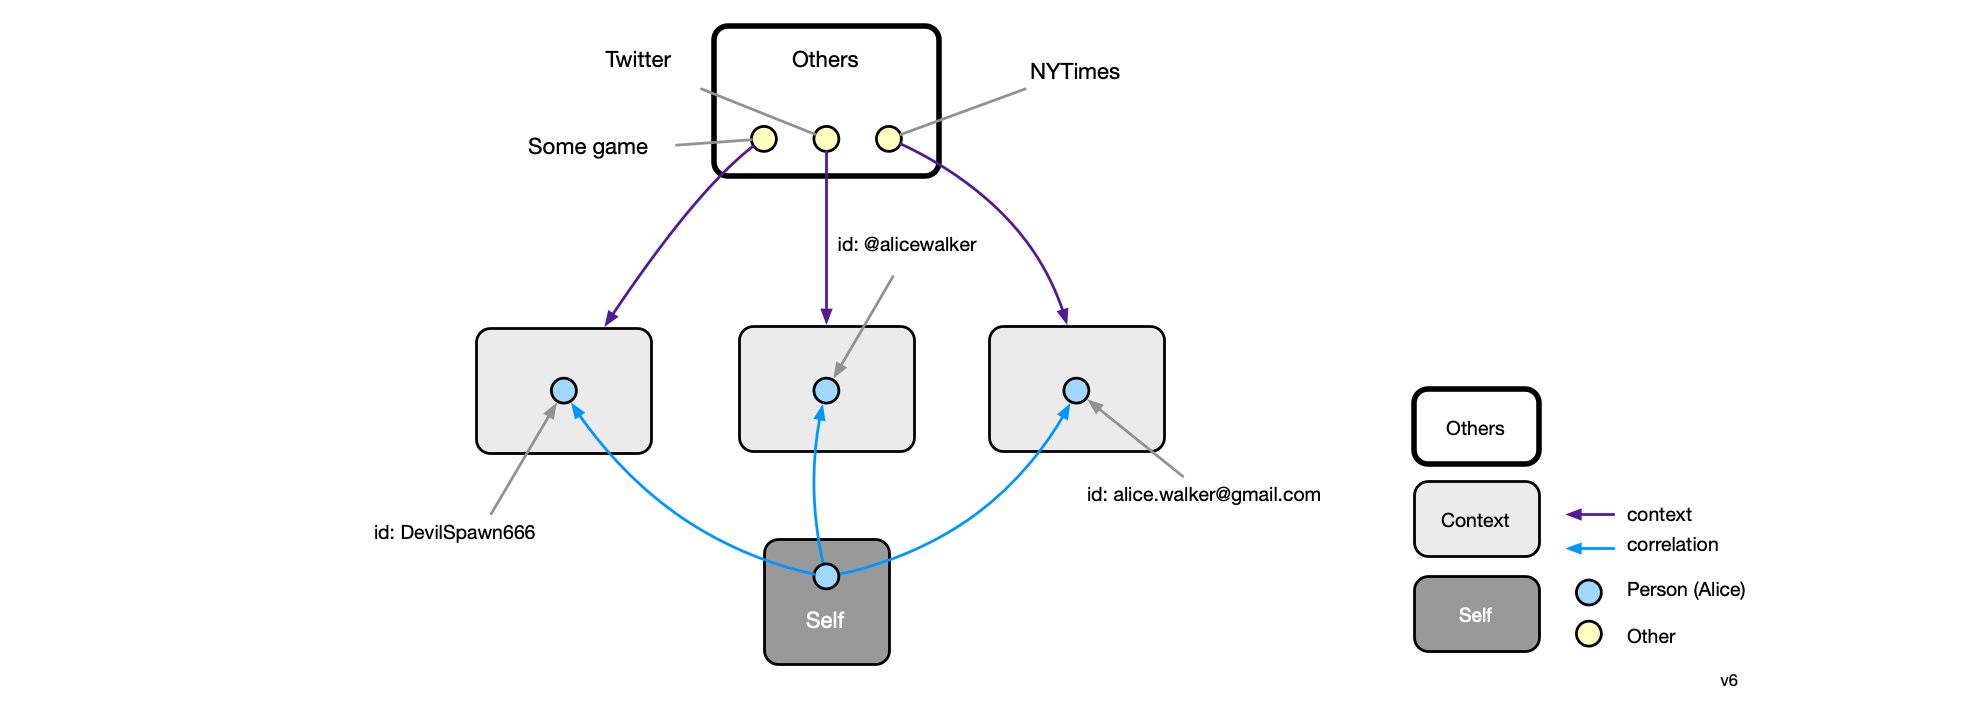
\includegraphics[width=\textwidth]{./images/example2.png}
\caption{Alices and Others}
\label{fig:Others-container}
\end{figure}

The personal data flowing through each of the three connections represented by the purple lines above may flow from the agent, to the agent, or in both directions. It may have originated on either side. It may be self asserted claims (attributes) entered by the user directly into the agent. Or it may be claims entered by the user on an app of the other party, or sensed by a local app (or sensor), or generated by the other party based on direct on-site or on-app interactions with the user.

\subsubsection{Container classes}

We describe the data model in two parts. The first part describes the data containers. The second describes the data that is held by those containers. Let us start describing the data model of the containers themselves. Figure~\ref{fig:containers} shows the various data container classes. 

\begin{figure}[h!]
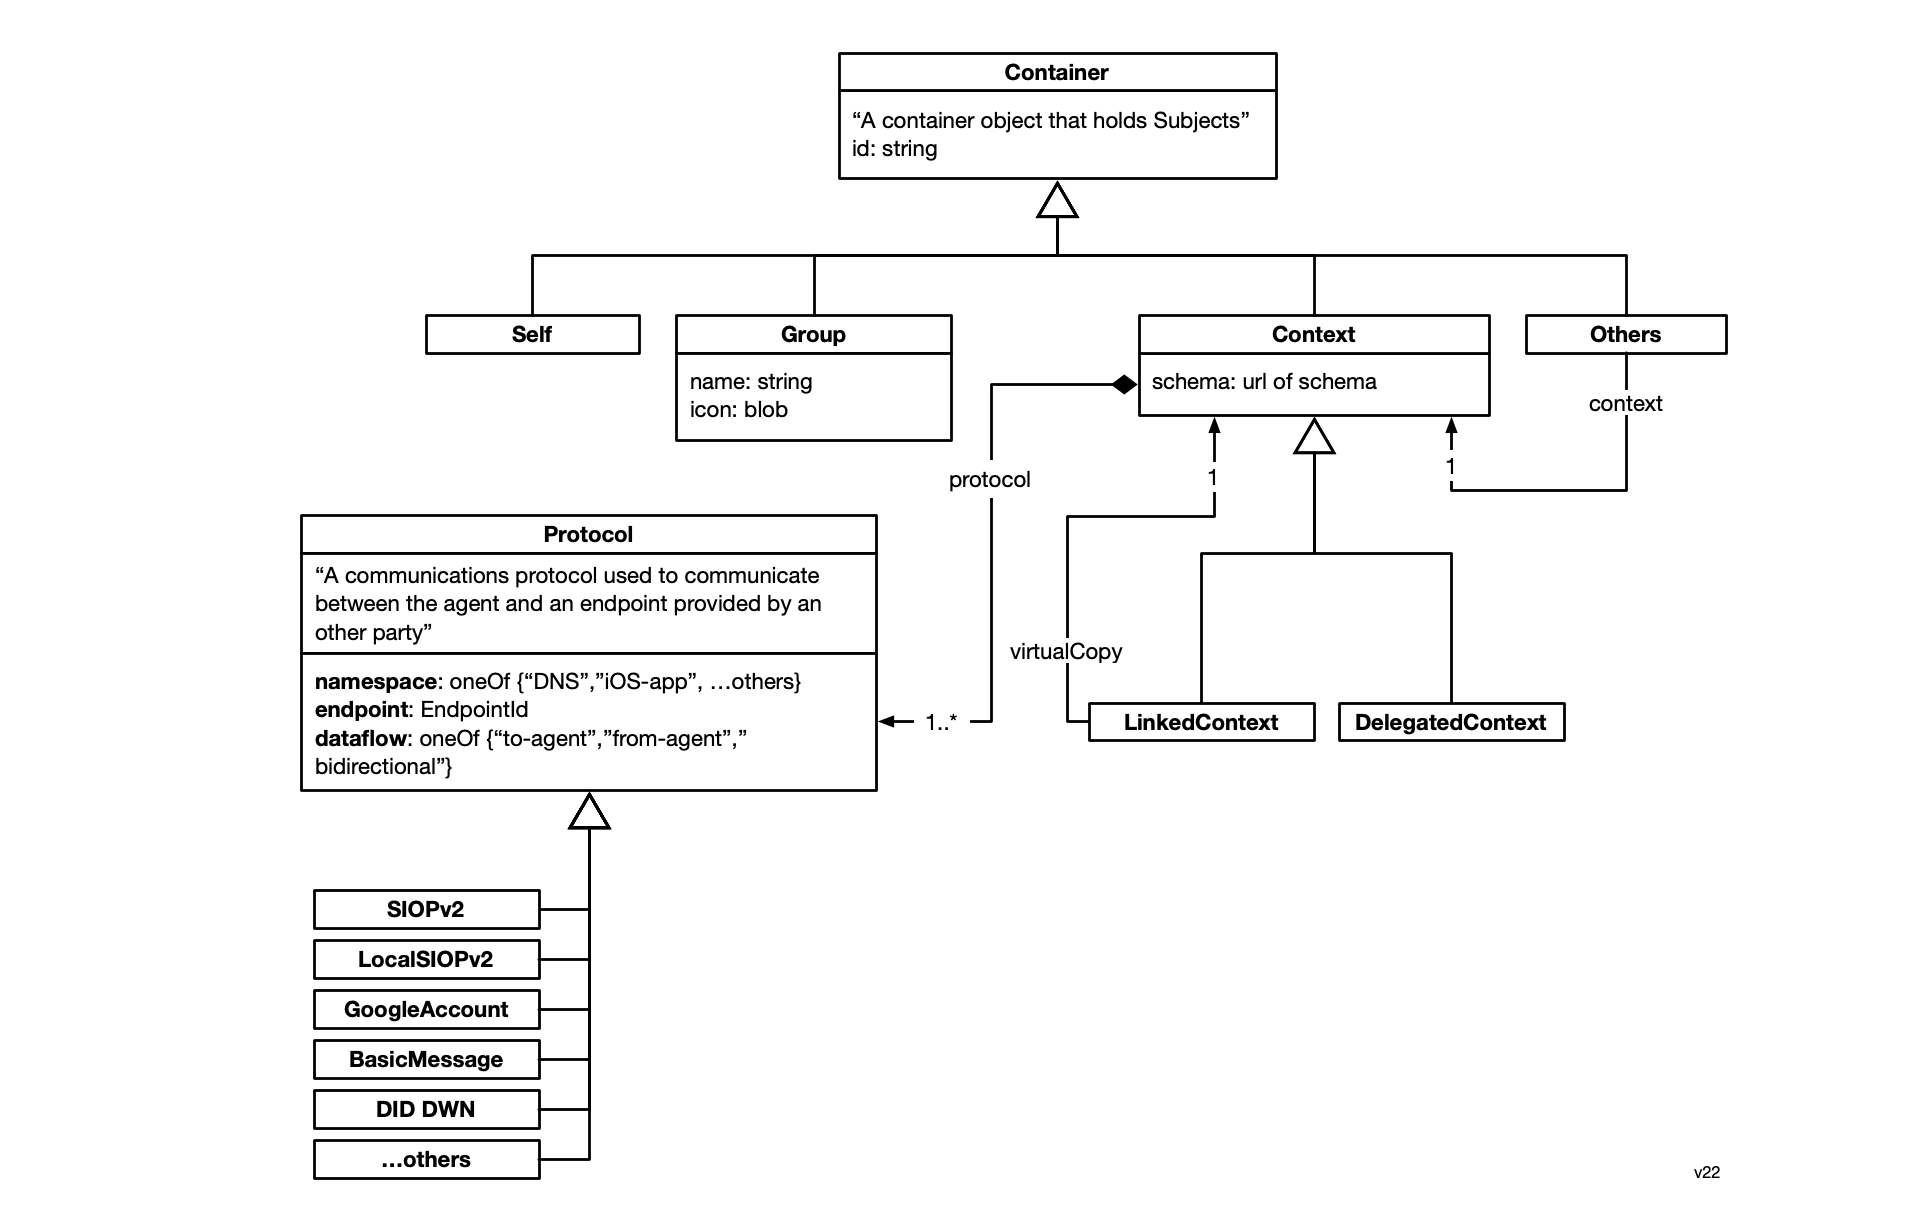
\includegraphics[width=\textwidth]{./images/container-classes.png}
\caption{Container classes}
\label{fig:containers}
\end{figure}

\textbf{Classes}

\begin{itemize}
\item \textbf{Others} - a container holding a set of Other nodes (see Persona Classes). Each Other node represents a party with the user has a connection. These Others may be other people or legal entities. If they are legal entities, they are often called relying parties, such as a digital service provider like Twitter, Inc. Each other has the following properties:
	\begin{itemize}
	\item \textbf{Context} - a single Context that captures one aspect of the overall connection
	\end{itemize}
\item \textbf{Self} - the single Container holding a single Person node that represents the selfness of the user
\item \textbf{Group} - an intermediate level container that holds a single Person node that represents a common role or persona that the user plays. A group has these attributes:
	\begin{itemize}
	\item \textbf{name} - the name of the group 
	\item \textbf{icon} - a icon for the group
	\end{itemize}
\item \textbf{Context} - a Container holding a Person node that represents the user in a specific aspect of their relationship with some other party. We say "specific aspect" because the relationship between the user a given other, may be represented by more than one context, each representing a different aspect. 
\end{itemize}

\textbf{More about Contexts}

A context has the following attributes, that taken together uniquely identify the context:

\begin{itemize}
\item \textbf{schema} - url of the schema of the data in the context
\item \textbf{protocols[]} - array of one or more Protocol instances
\end{itemize}

The kinds of data held by a context depends on the communications protocol (using the term loosely) between the agent and the other party. As will be described next, a Protocol class within the agent represents these data conventions using a schema that is an extension of the Persona schema.

There are two subclasses of Context: \emph{LinkedContext} and \emph{DelegatedContext} that are described in their own sections below.

\textbf{Protocols}

A Protocol class represents a communication protocol used between the agent and an endpoint provided by an other party. Each protocol subclass represents a different communications protocol such as SIOPv2, GoogleAccountSync, BasicMessage (DIDComm), etc.  Protocol classes have a class method that returns the data schema used when it updates data in that context. These schemas are resolvable from a URL which is written to the *schema* attribute of the Context instance.

A Protocol is an attribute of a Context, and although a less common situation, may have more than one. Figure!\ref{fig:protocol} shows an example of a user Alice who has a (hypothetical) connection with Santander Bank. This connection has a single context that contains the information that Alice shares in with the bank via the OpenID Connect SIOPv2 protocol.

\begin{figure}[htbp]
	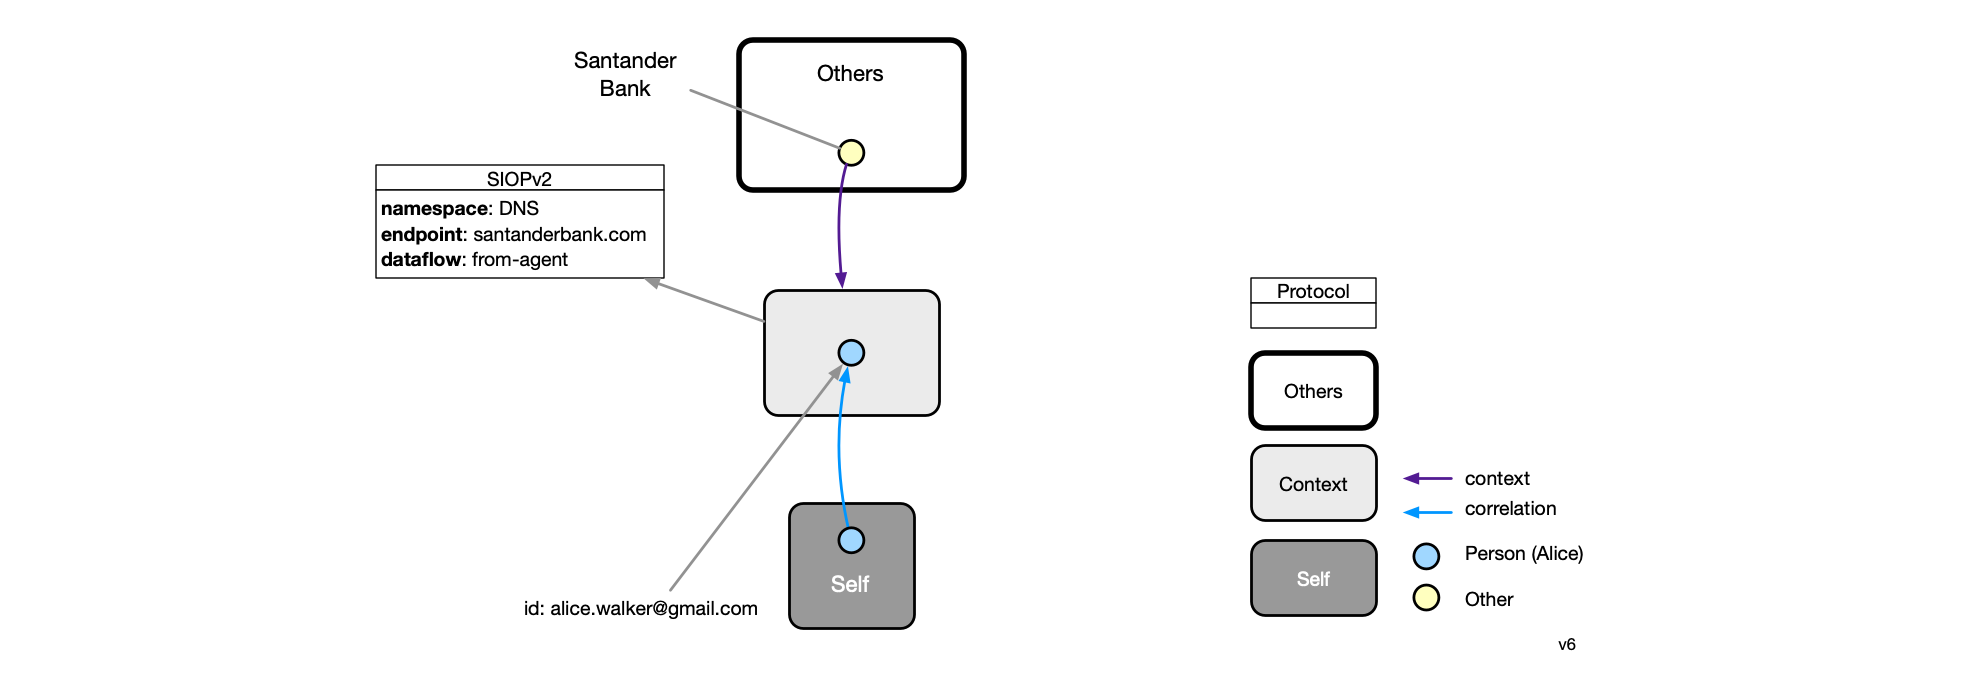
\includegraphics[width=\textwidth]{./images/context-with-protocol.png}
	\caption{Protocols}
	\label{fig:protocol}
\end{figure}

Each protocol instance has these attributes:
\begin{itemize}
\item \textbf{namespace} - a string that indicates the namespace used by the ``endpoint" attribute
\item \textbf{endpoint} - a string identifier that unique identifies the other party with which the user has a relationship within the above namespace attribute
\item \textbf{dataflow} - one of {to-agent, from-agent, bidirectional} - indicates the direction of data flow between the agent and the endpoint
\end{itemize}

\textbf{Multiple connections}

In the example shown in figure~\ref{fig:groups}, we expand our story about Alice. Now she has defined two groups. The first represents her role as a journalist, and it contains two contexts: the context representing her relationship with Google and with Twitter. The Google context contains her Google account profile which can be updated either using her agent or via the Google website (hence the ``bidirectional" dataflow). Her Twitter context contains a snapshot of all of her Twitter account information, lists of who she follows, etc. 

The second group, entitled ``News" contains a Person linked to three contexts all belonging to the New York Times. The first of these three is the context that she uses, via SIOPv2 to login to the NYTimes website. The second is a context that contains data her form filler Safari extension uses. The last is a context that establishes a bidirectional connection with the NYTimes using a new (and purely hypothetical for now!) bidirectional data synchronization protocol called MeeTalk. She plays a game for which there is a context (without being within an intervening Group), and she has a direct relationship with her friend Bob using the DIDComm BasicMessage protocol.  

\begin{figure}[htbp]
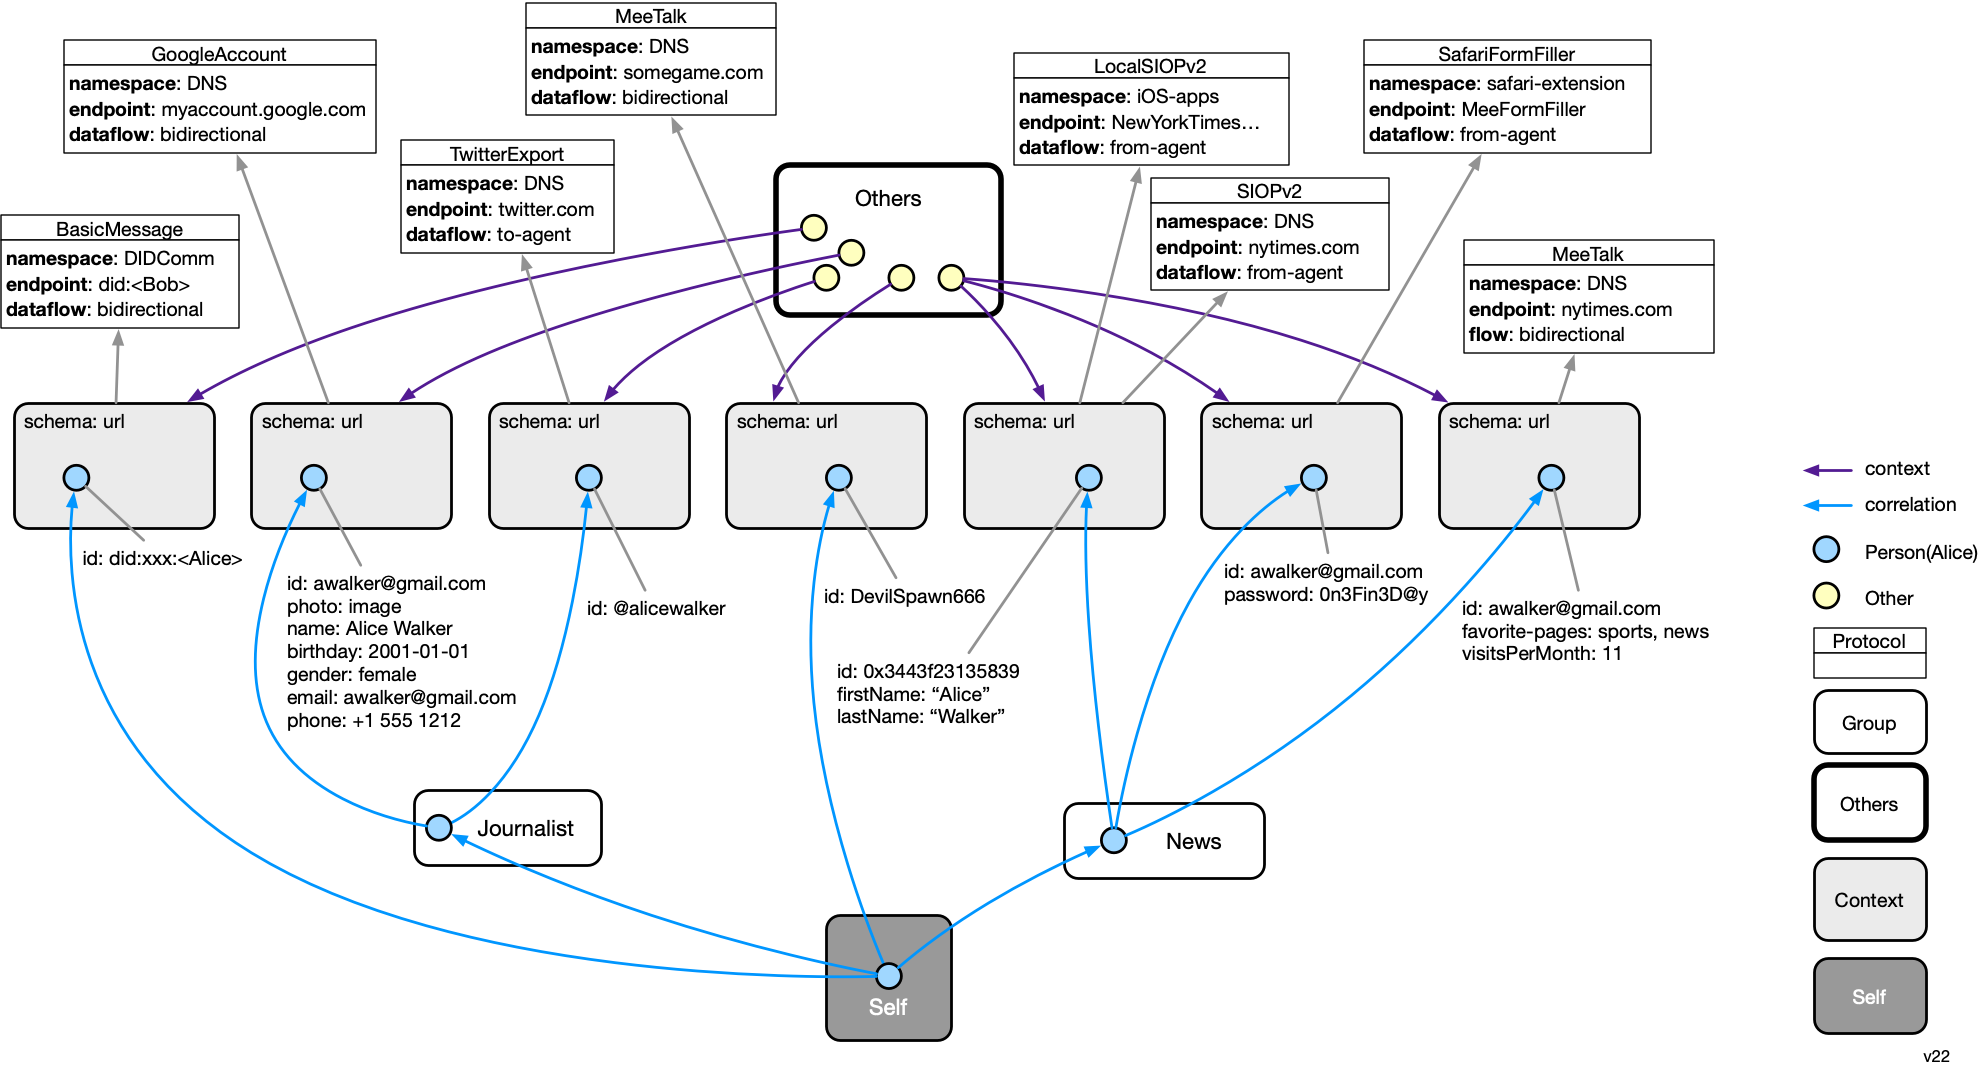
\includegraphics[width=\textwidth]{./images/multiple-connections.png}
\caption{Alice with two groups of connections}
\label{fig:groups}
\end{figure}

A relationship between the identity agent and another party is called a \emph{Connection}. It is represented by one or more other contexts each of which has a protocol (and sometimes more than one). Alice is shown with five connections--one for each of the five Other nodes in her Others container. 

\textbf{Linked contexts}

Alice can convey claims made about her by one party and present them to another party. For this example we'll assume that the claims are encapsulated within a \hyperfootnote[Verifiable Credentials][https://]{w3.org/TR/vc-data-model/} document. 

\begin{figure}[htbp]
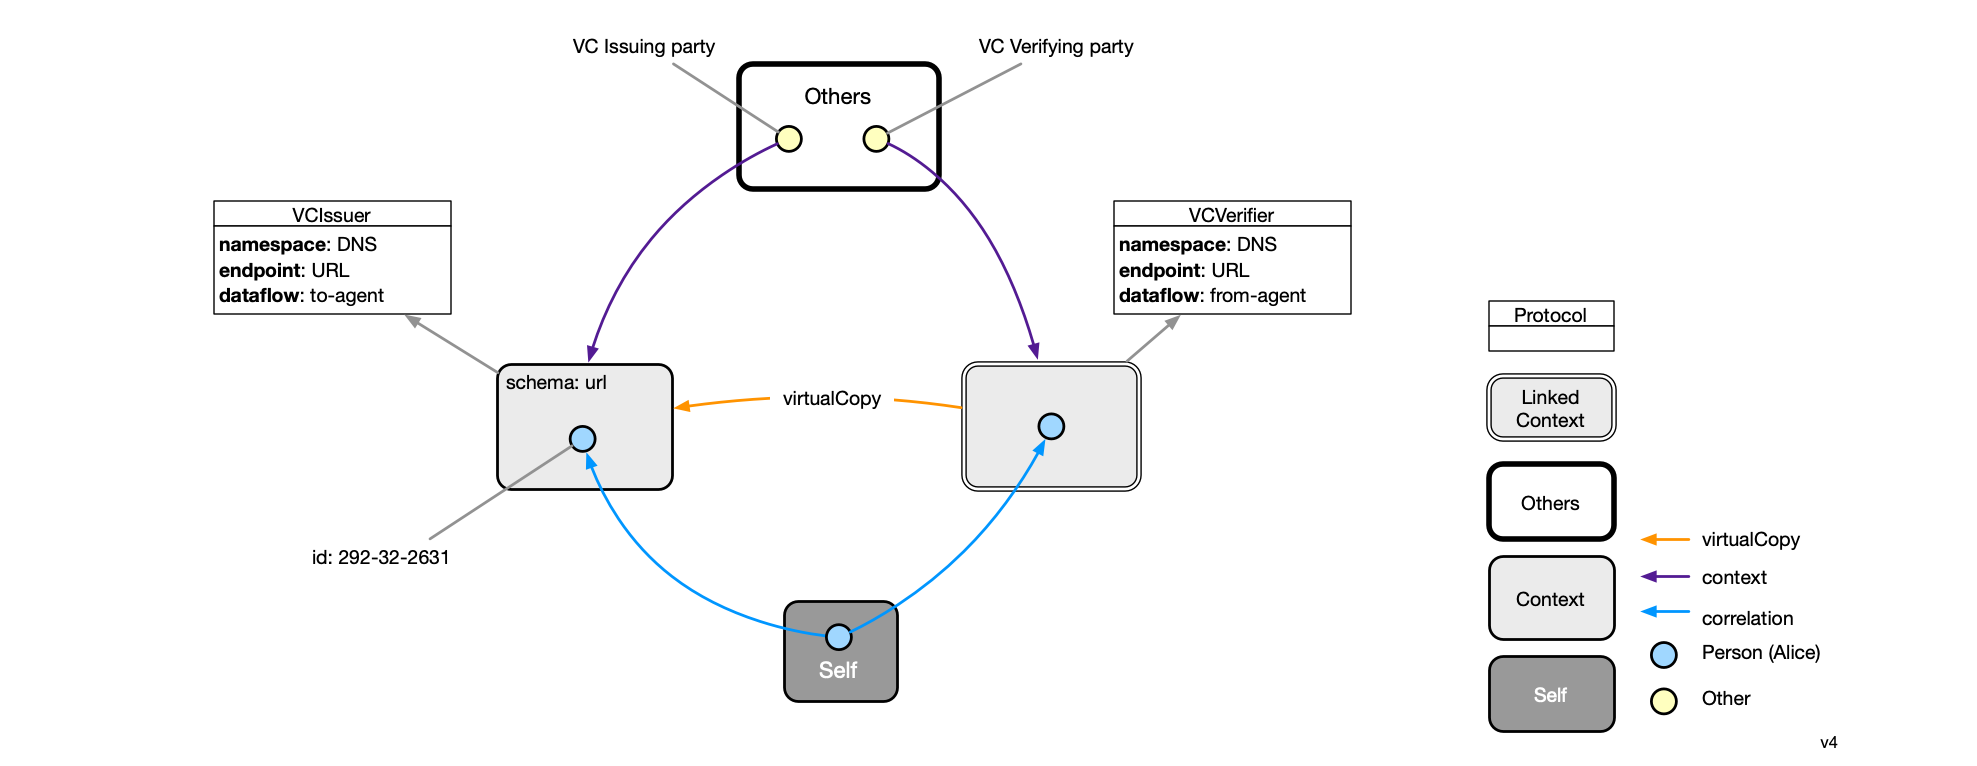
\includegraphics[width=\textwidth]{./images/linked-contexts.png}
\caption{Linked Contexts}
\label{fig:linked-contexts}
\end{figure}

In this example Alice shown in in figure~\ref{fig:linked-contexts}, presumably having authenticated herself in her connection to an app of the ``VC Issuing party" is issued a VC containing claims about her which is stored in the leftmost context above. She then goes to another app of the ``VC Verifying party" and finds that they trust the issuing party and thus would accept a VC issued by them. In Alice's second connection a VC presenting protocol is used to send the VC to the verifying party. This second connection involved a special class of context, called a \emph{LinkedContext}. 

\textbf{Delegated contexts}

Alice takes care of her elderly mother, and helps her mother manage her bank account at Santander Bank. Alice's mother has an agent containing a connection to her bank, the data for which (e.g. her mother's OpenID Connect SIOP claims) is stored in one of the contexts representing this connection. Using her agent, Alice's mother has delegated access to this context to her daughter Alice.

\begin{figure}[htbp]
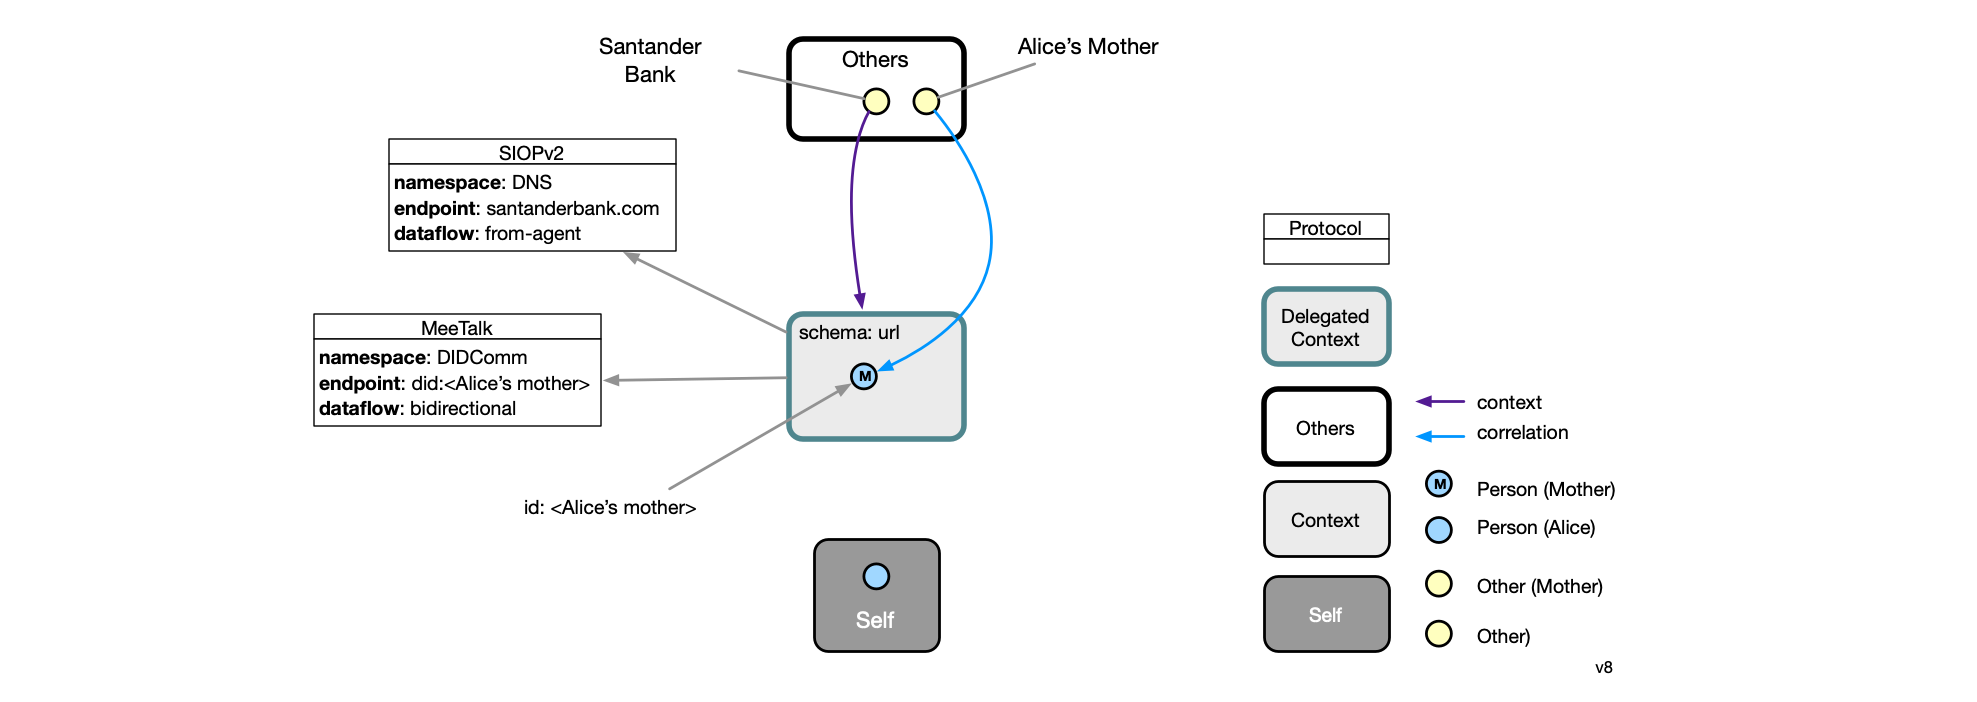
\includegraphics[width=\textwidth]{./images/delegated-contexts.png}
\caption{Alice's agent with a connection using a delegated context}
\label{fig:delegated-contexts}
\end{figure}

As shown in figure~\ref{fig:delegated-contexts}, Alice's mother's connection with her bank is represented by a delegated context. Alice now has the ability to view (and potentially update) information in this context. Information about Alice's mother's account information at the bank might be helpful for Alice to have while taking care of her mother. Data replication/synchronization is used to ensure that Alice's DelegatedContext is always synchronized with the ``original" context on her mother's agent.

Whereas the main point here is giving Alice visibility into her mother's bank, information, it may be possible in some cases for Alice's agent to use this information to authenticate as her mother to the bank (although authenticating as someone else (especially in the case of abank) is usually a violation of the terms of service of the other party.

\subsubsection{Persona classes}

Group and context containers contain information about subjects (things) that are described according to the \emph{Persona} schema. In knowledge representation parlance, the Persona schema would be known as an \emph{upper ontology}.

In the Persona schema, people are be represented as instances of Person, a \emph{PersonalAccount} class is also defined. These classes are shown below. 

\begin{figure}[htbp]
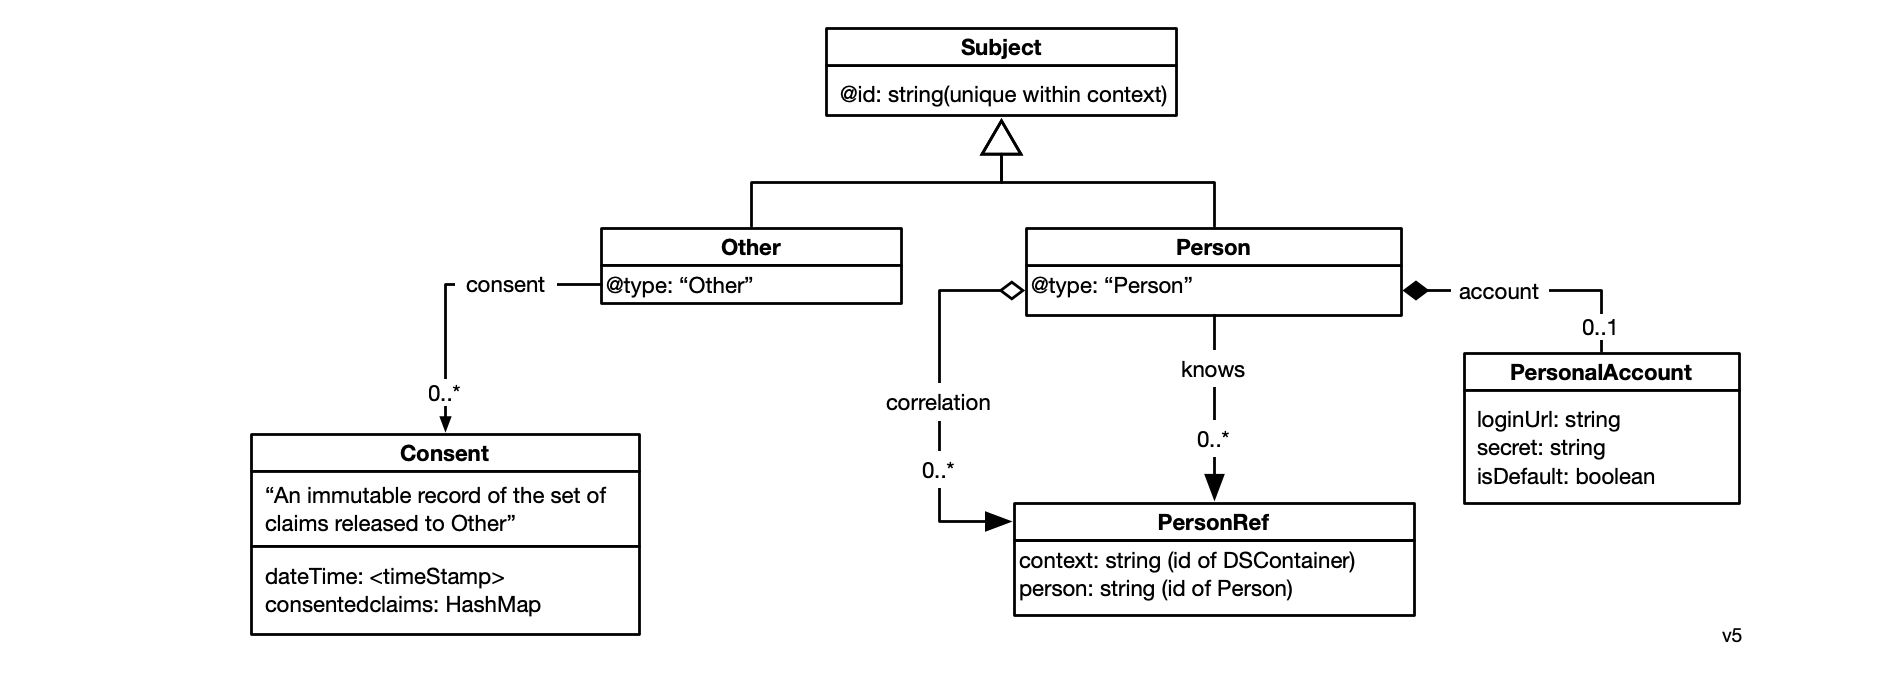
\includegraphics[width=\textwidth]{./images/persona-classes.png}
\caption{Persona schema}
\end{figure}

\textbf{Classes}

\begin{itemize}
\item \textbf{Subject} - kind of digital subject about which the agent stores information
\item \textbf{Person} - a natural person, a subclass of Subject. Each person has the following properties:
	\begin{itemize}
	\item \textbf{claims[]} - a set of zero or more properties. Here are a few examples: 
		\begin{itemize}
		\item givenName
		\item familyName
		\item phoneticGivenName
		\end{itemize}
	\item \textbf{account} - an optional PersonalAccount at some other party's site or app
	\item \textbf{correlation} - zero or more PersonRefs that act as a link to a target Person object representing another whoness of the link's source's person's selfness.
	\item \textbf{knows} - zero or more PersonRefs that link to a Person representing some other person (other than the user)
	\end{itemize}
\item \textbf{Other} - a Subject representing another person or a legal entity with which the user has a connection. Each Other object has:
	\begin {itemize}
	\item \textbf{consents} - zero or more Consent objects. Each Consent has:
		\begin{itemize}
		\item \textbf{dateTime} - time stamp of when the user consented to share this set of claims
		\item \textbf{claims[]}  - a set of zero or more claims (note: claim types (e.g. ``email address") not their values)
		\end{itemize}
	\end{itemize}
\end{itemize}

\textbf{Extensions}

Each protocol class will extend the Persona schema by defining Person subclasses, other new object classes and new kinds of relationships. For example the Google
\hyperfootnote[Google Account][https://]{myaccount.google.com}  API includes (optional) claims of ``name", ``gender" and ``birthday". The protocol that supports the myaccount API would define these claim types in its schema, and insert a link to this schema in its corresponding context's \emph{schema} attribute.

\subsubsection{Datatypes}

This section is largely incomplete, but will eventually describe lower level classes that we call \emph{datatypes} that are used by the higher level classes mentioned above. Some datatype classes are shown in figure~\ref{fig:datatypes}.

\begin{figure}[htbp]
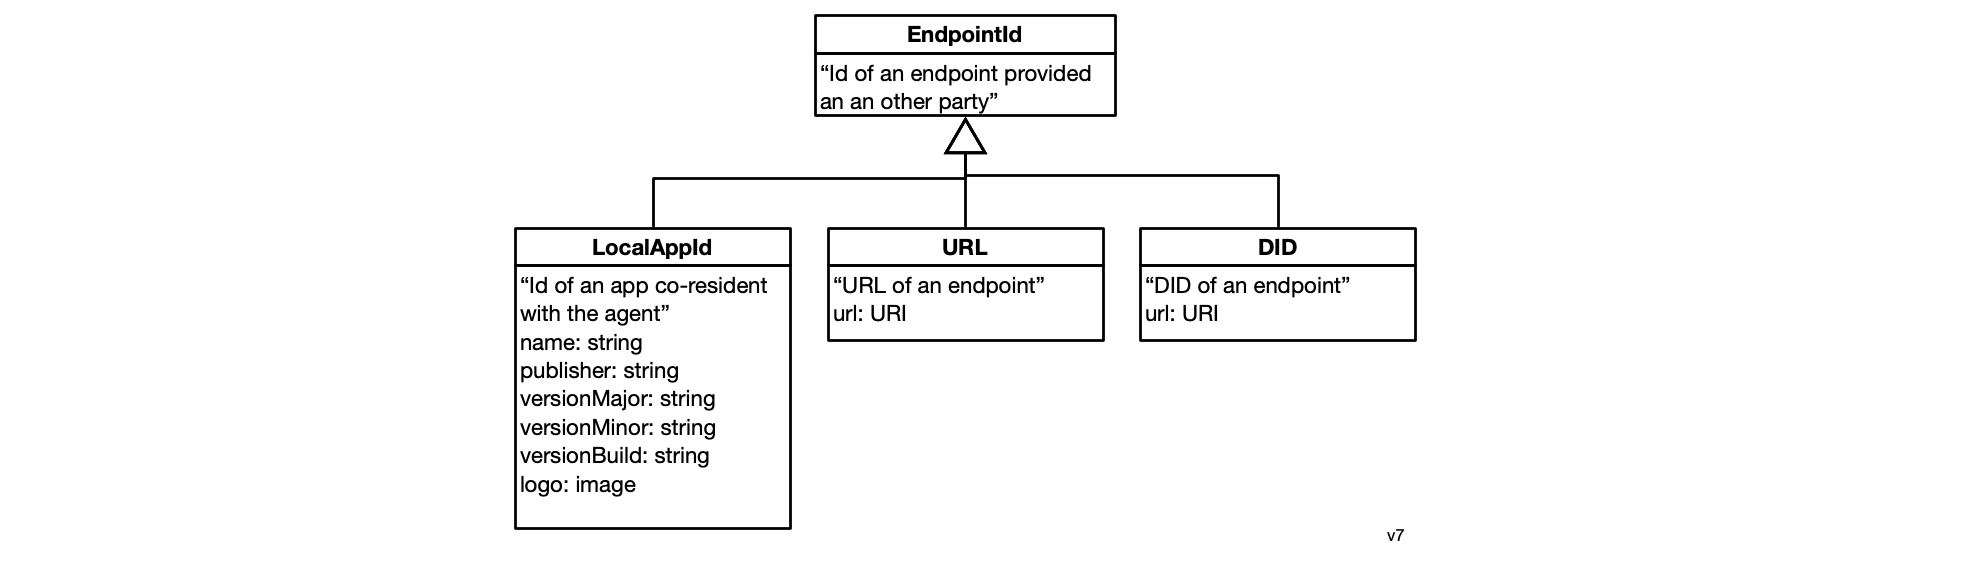
\includegraphics[width=\textwidth]{./images/datatypes.png}
\caption{Datatypes}
\label{fig:datatypes}
\end{figure}

\begin{itemize}
\item \textbf{EndpointId} -  an identifier of an endpoint (e.g. webservice or a local app) supported by an other party.
\item \textbf{LocalAppId} - A specific kind of EndpointId. Uniquely identifies a service provider's mobile app. 
\item \textbf{Secret Recovery Phrase} - a 12-word textual phrase that the user creates. It is used to generate cryptographic keys that in turn are used to encrypt the user’s personal data whether it is stored locally on their device or in a backup location. It can be used to generate keys to digitally sign transactions (e.g., for crypto currency transactions). It should never be shared with anyone or any service provider. If the user loses this phrase, they lose the ability to decrypt their data. 
\end{itemize}

\section{Agents and apps} % SECTION 

We turn now to interactions between an agent and apps. 

\subsection{Private data sharing}

Data held and/or managed by the user's agent and stored on-device, is inherently under the user's control. Data that the user shares with another party or is collected by them in other ways \emph{also} needs to be under their control. Since no technical means exist to control data held by another party, we rely on law. Current privacy laws and regulations are intended to provide this control, but as we've discussed, place such burdens on the user to effectuate their control that in practice this control hardly exists. The solution we proposed is to combine both legal (license agreement) and technical means (identity agents). 

The legal mechanism we propose is the \hyperfootnote[Human Information License (HIL)][https://]{docs.google.com/document/d/13aGk5adoncMxxfl5637NfqP6fl6q\_op\_1CF50UrJNjg}. The (HIL) is a contract between two parties. The first is the digital service provider. The second is a nonprofit, organization called The Mee Foundation (TMF), that represents the community of agent users. The TMF is a \emph{Mediator of Individual Data} (MID), a term coined by Lanier et al.\cite{Lanier2018}, that enforces the terms of the HIL on behalf of the user community. 

The HIL imposes obligations on the provider. Among them is the provider's requirement to respect the user's \emph{data rights} to access, correction (editing), and deletion of the information collected and held by them. It covers information that the user may have shared information manually (e.g. by filling in a form, or other kinds of on-app interactions) or shared with them by a user's agent. The HIL requires the provider to implement \emph{data rights} APIs that an agent uses to remotely control this app-held data. In this way, we tie the legal (HIL) and technical means (agents and APIs) together.

The HIL's provisions are intentionally generic. They are designed to meet the needs of the entire community of agent users. We expect that other contracts containing more specific provisions will be required to meet the needs of more specialized communities. Groups of user communities can amend the HIL to meet the specifics they require, provided that they do not weaken the HIL's existing provisions and protections. These specialized communities would organize, govern and operate independent MIDs that enforce their more specialized HIL-based contracts. These specialized MIDs would enter into agreements with one or more providers which would be held to both the generic terms of the HIL as well as the additional, specialized terms.

\subsection{App-Agent Interactions}

In figure~\ref{fig:interactions} we show Alice's agent in the \emph{Agent} layer is interacting with apps in one of two \emph{Application Layers}. The top application layer contains two apps running on a remote system. The first is \emph{Bob's Agent} which appears to Alice as an app (just as, by symmetry, Alice's agent appears as an app to Bob's agent). The second is a website labeled \emph{Provider's Website}. The lower application layer contains \emph{local apps} that run on the same device where Alice's device agent is also running. The digram shows a local app labelled \emph{Provider's Local App}.

\begin{figure}[htbp]
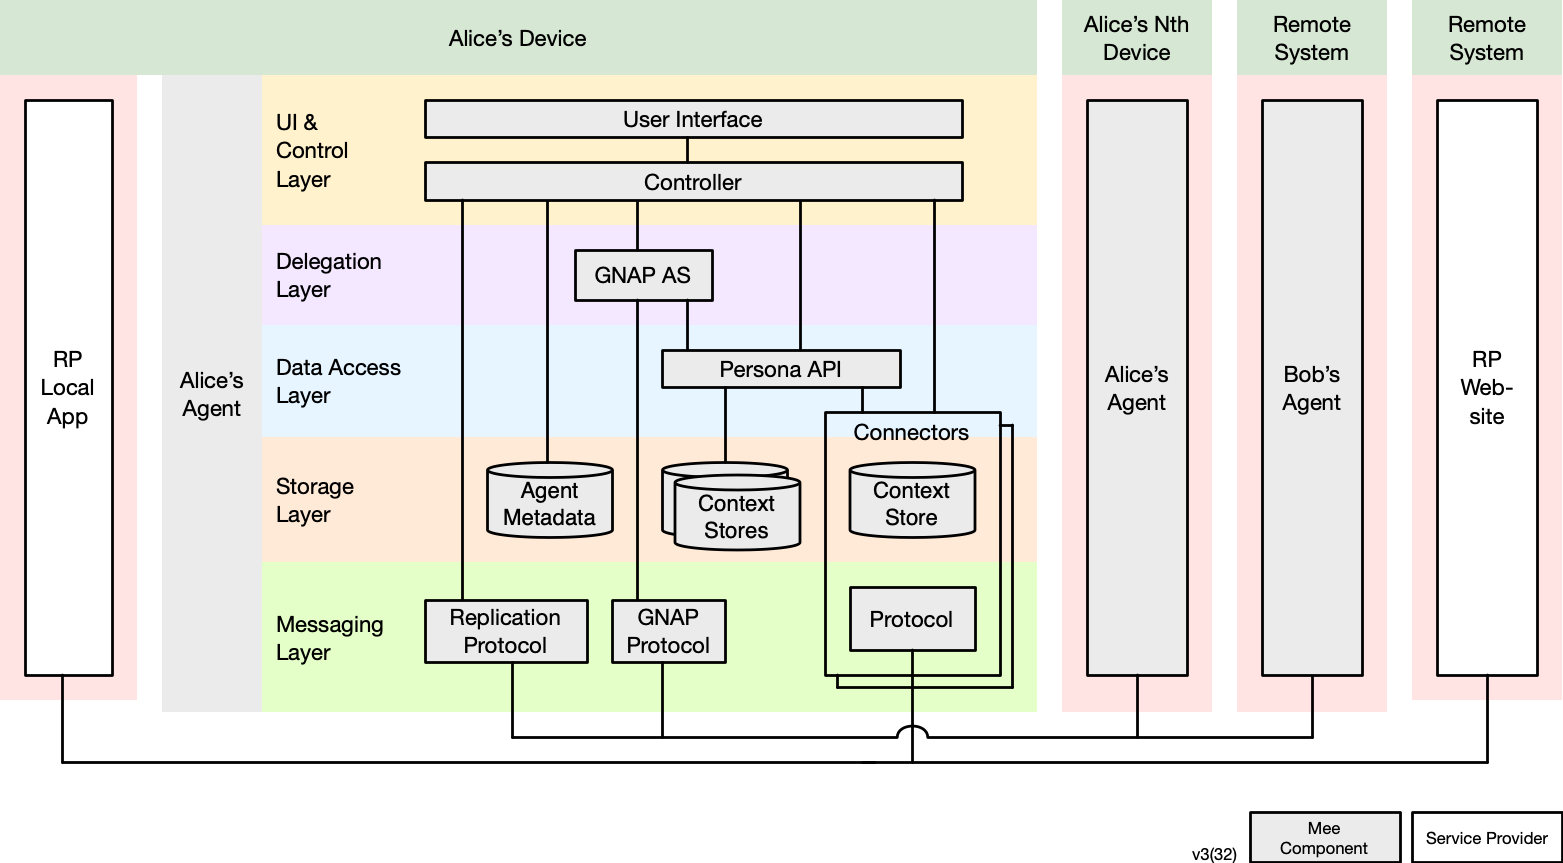
\includegraphics[width=\textwidth]{./images/applications.png}
\caption{Identity agent interactions with apps}
\label{fig:interactions}
\end{figure}

There are four types of intereactions between an app and an agent:
\begin{enumerate}
	\item \textbf{Request} - app needs information from the agent
	\item \textbf{App-initiated Sync} - app has updated information to sync with the agent
	\item \textbf{Agent-initiated Sync} - agent has updated information to sync with the app
	\item \textbf{Delete Context} - user has directed their agent to delete a connection and all of its associated contexts
\end{enumerate}

\textbf{Request}

When a user uses an app, the app may at one or more points in the interaction need information about the user. The information requested is usually information about the user, but not could be about other people or any other topic. The information requested may be a simple list of attributes and values, or something more complicated. The app can express whether the information is required or optional.

The concept of \emph{authentication} is a kind of request wherein the app wants to know the identity of the user so it can know if this a new user, or a previous user from the past so as to influence authorization decisions. In a traditional app, an authentication request is implemented using a user login/sign-in interaction. In an agent-based architecture, a \emph{request} message can be used for this purpose. To initiate a request the user taps a \emph{Mee} button on the app to initiate a request for information. This tap initiates an \hyperfootnote[OpenID SIOPv2][https://]{openid.net/specs/openid-connect-self-issued-v2-1\_0.html} \emph{Authorization Request}. In the narrow context of authentication the information requested and returned are often called \emph{claims} since they are usually claims made by some entity (possibly the user) about the user.

Beyond authentication, the app may send a request for information to the user's agent by displaying the Mee button as needed during an interactive session. 

Figure \ref{fig:request} shows the \emph{request} interaction in a bit more detail. The agent receives the request message which contains a query describing the kind of information required and/or desired. The agent searches for relevant objects and/or attributes in its storage layer. The agent then does the some or all of the following:
\begin{enumerate}
	\item \textbf{Discuss with user.} Depending on the search results for the information, the agent and the user may need to discuss what object and/or attribute values to return. For example, if two conflicting values are found for the same attribute type, the agent may wish to ask the user which (if either) they would like to disclose. If zero or one values are found for a given claim then this step can be skipped, at least for this claim.
	\item \textbf{Update context.} Populate the context container with the claims (if any) returned from the search.
	\item \textbf{Display consent screen.} Agent displays consent screen pre-filling what it can and allowing the user to fill in the rest. 
	\item \textbf {Create consent object.} Agent records this consent event.
\end{enumerate}

In the response to the \emph{request} message, the agent returns a non-correlatable \emph{contextId} that can be used for future app-initiated sync operations.

\begin{comment}
title Request
App->Agent:request
Agent->AgentStorage:cross-context query
Agent<-AgentStorage:results
note over Agent:Discuss with user
note over Agent:Update context 
note over Agent:Display consent screen
note over Agent:Create consent object
App<-Agent:response
\end{comment}

\begin{figure}[htbp]
	\centering
	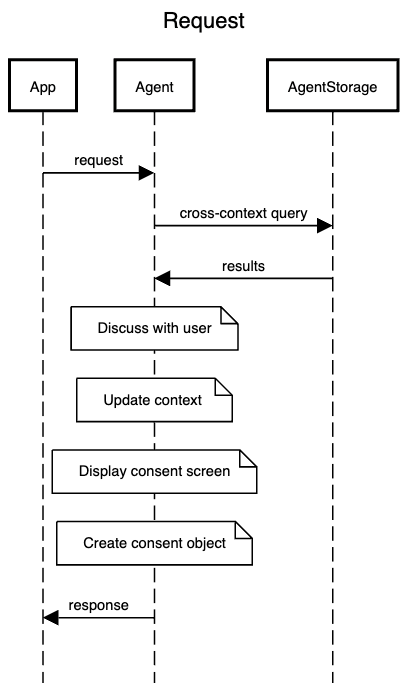
\includegraphics[width=0.50\textwidth]{./images/int-request.png}
	\caption{Request}
	\label{fig:request}
\end{figure}

\textbf{App-Initiated Sync}

Apps are required to sync to the agent any changes to claim (aattribute) values, as well as any new attribute values. For example, if the user were to use a webform on the app to update and existing or add a new shipping address, then this information must be synced to the agent. This app-initiated sync operation is shown in figure \ref{fig:app-initiated_sync}.

\begin{comment}
title App-Initiated Sync
App->Agent:sync(contextId, updates)
note over Agent:Update context
Agent->App:return
\end{comment}

\begin{figure}[htbp]
	\centering
	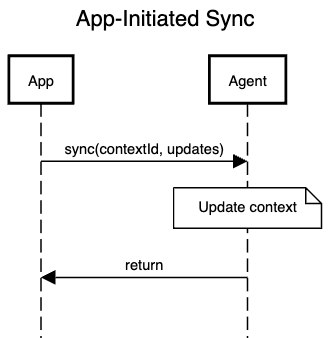
\includegraphics[width=0.33\textwidth]{./images/int-app-initiated_sync.png}
	\caption{App-Agent Interactions: App-Initiated Sync}
	\label{fig:app-initiated_sync}
\end{figure}

\textbf{Agent-Initiated Sync}

When the user is interacting with other apps (i.e. apps other than the current one) a new value of a attribute is generated or captured that perhaps should be updated within the current app context. In this case (given appropriate prior consent by the user) an update value of this claim can be automatically synced from the agent to the app. Figure \ref{fig:agent-initiated_sync} shows this flow. The agent sends one or more sync messages to the app related to the contextId of the current context.

\begin{comment}
title Agent-Initiated Sync
Agent->App:sync(contextId, updates)
App->Agent:response
\end{comment}

\begin{figure}[htbp]
	\centering
	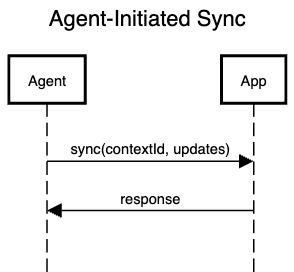
\includegraphics[width=0.33\textwidth]{./images/int-agent-initiated_sync.png}
	\caption{Agent-Initiated Sync}
	\label{fig:agent-initiated_sync}
\end{figure}

\textbf{Context Deletion}

There is one final app-agent interaction, namely, \emph{context deletion}. This occurs whtn the user choses a connection on their agent and taps ``Delete.'' As shown in figure \ref{fig:context-deletion}
the agent initiates deleteContext messages for each context within the connection.

\begin{comment}
title Delete Context
Agent->App:deleteContext
App->Agent:return
\end{comment}

\begin{figure}[htbp]
	\centering
	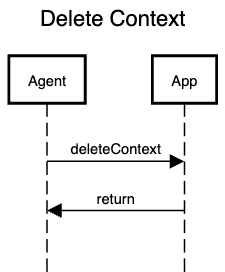
\includegraphics[width=0.33\textwidth]{./images/int-context_deletion.png}
	\caption{Context Deletion}
	\label{fig:context-deletion}
\end{figure}

\clearpage

\section{Acknowledgements}
Contributors to this paper include Kiril Khalitov, Sergey Kucherenko, Maria Vasuytenko, and Alexander Yuhimenko.

\bibliography{../library}
\bibliographystyle{plainurl}


\end{document}  